% trim={5cm 0 0 0},clip

{\let\clearpage\relax\let\cleardoublepage\relax
\chapter{Sistema solare}
}
Il sistema solare \'e il punto di partenza delle teorie di formazione planetaria. Infatti si hanno informazioni accurate sui pianeti e loro orbite e sulla popolazione di corpi minori, si hanno anche riferimenti temporali tramite analisi chimica di campioni di roccia.

L'et\'a del sole \'e definita come tempo in sequenza principale; tecniche eliosismologiche determinano un'et\'a di \SI{4.57+-0.11}{\giga\year} mentre l'analisi chimica dei meteoriti \SI{4.57+-0.07}{\giga\year}.
La Terra si \'e formata completamente circa \SI{100}{\mega\year} dopo i meteoriti.

\begin{figure}[!ht]
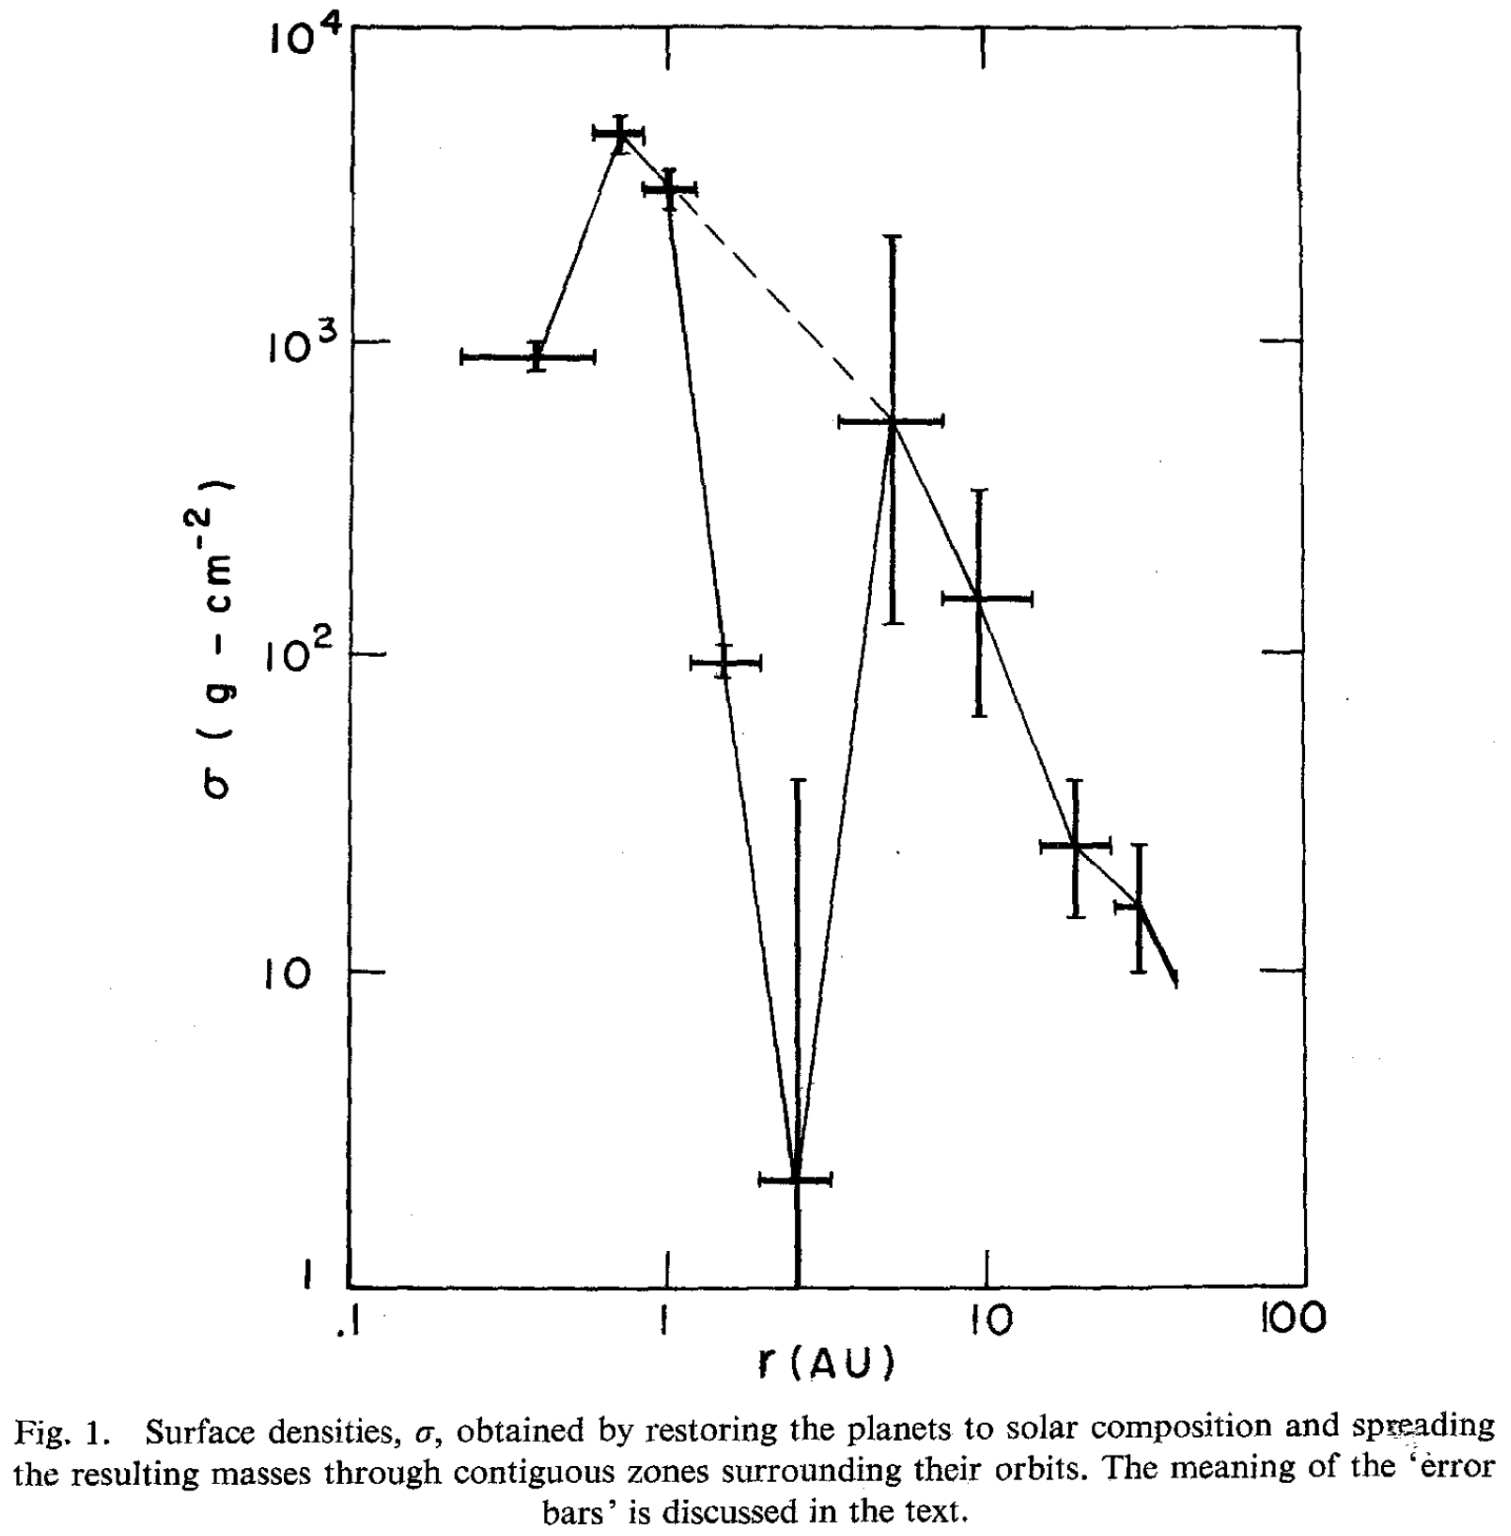
\includegraphics[trim={0cm 5cm 0 0cm},clip, width=0.9\textwidth]{Snebuladensity}\caption{Andamento minimum mass solar nebula (MMSN). Da \cite{weidenschilling1977distribution}.}\label{fig:Snebuladensity}
\end{figure}

Per stimare la massa del disco protoplanetario \cite{weidenschilling1977distribution} ha considerato la massa presente nei pianeti e nella fascia asteroidale arricchita di H/He per avere composizione solare: distribuendo questa massa in un anello di spessore proporzionale al raggio di Hill e centrato sulle orbite si ha l'andamento della densit\'a superficiale mostrato in figura \ref{fig:Snebuladensity}. \cite{hayashi1981structure} ha determinato l'andamento della densit\'a di gas, ghiaccio e rocce:
%$\Sigma\propto r\expy{-3/2}$.
\begin{align}
&\Sigma_{rock}=7.1(\frac{a}{\si{\astronomicalunit}})\expy{-3/2}\si{\gram\per\square\cm}:\ \frac{a}{\si{\astronomicalunit}}=0.35-2.7\\
&\Sigma_{rock+ice}=30(\frac{a}{\si{\astronomicalunit}})\expy{-3/2}\si{\gram\per\square\cm}:\ \frac{a}{\si{\astronomicalunit}}=2.7-36\\
&\Sigma_{gas}=\num{e3}(\frac{a}{\si{\astronomicalunit}})\expy{-3/2}\si{\gram\per\square\cm}:\ \frac{a}{\si{\astronomicalunit}}=0.35-36
\end{align}

\begin{workout}[accrescimento di gas su nucleo solido prevede arricchimento di metalli ]

\end{workout}

%La formazione per accrescimento di gas su nucleo solido prevede arricchimento di metalli rispetto alla composizione di partenza.
Vincoli alla distribuzione di massa interna sono imposti dalla misura dei momenti di multipolo del potenziale gravitazionale: risolvendo un modello di pianeta che rientri nei vincoli osservativi si determinano la massa del core e la metallicit\'a dell'inviluppo gassoso dei 4 pianeti gassosi (vedi  tabella \ref{tab:JSUNcomp}).

\begin{table}[!htb]
    \begin{minipage}{.5\linewidth}
      \centering
        \begin{tabular}{|ccc|}
\hline
&\parbox{1.5cm}{Jupiter $317.8\mearth{}$}&\parbox{1.5cm}{Saturn $95.1\mearth{}$}\\
  $M_c$&$0-11\mearth{}$&$9-22\mearth{}$\\
\hline
$M_Z$&$1-39\mearth{}$&$1-8\mearth{}$\\
\hline
$M_Z^{tot}$&$8-39\mearth{}$&$13-28\mearth{}$\\
\hline
$Z/Z_{\odot}$&$1-6$&$6-14$\\
\hline
 \end{tabular}
    \end{minipage}%
    \begin{minipage}{.5\linewidth}
      \centering
        \begin{tabular}{|ccc|}
\hline
&\parbox{1.5cm}{Uranus $14.5\mearth{}$}&\parbox{1.5cm}{Neptune $17.1\mearth{}$}\\
\hline
$M_{rock}$&$3.7\mearth{}$&$4.2\mearth{}$\\
\hline
$M_{ice}$&$9.3\mearth{}$&$10.7\mearth{}$\\
\hline
$M_{H/He}$&$1.5\mearth{}$&$2.2\mearth{}$\\
\hline
        \end{tabular}
    \end{minipage} 
    \caption{Composizione Giove, Saturno, Urano e Nettuno. Da \cite{baraffe2009physical}.}\label{tab:JSUNcomp}
\end{table}

Modelli pi\'u sofisticati impongono vincoli maggiori sulle condizioni iniziali: il modello di Nizza del sistema solare (\cite{tsiganis2005origin}) riproduce caratteristiche orbitali dei pianeti giganti considerando la loro migrazione in una distribuzione di planentesimi di $30-50\mearth{}$; la presenza di numerosa popolazione di planetesimi \'e corroborata dalla craterizzazionedei pianeti terrestri e corpi minori come dall'esistenza di numerosi oggetti di piccole dimensioni superstiti.

\begin{workout}[Cosa dire dei modelli planetarii: core giganti gassosi: modelli planetari e raffronto isolation mass in MMSN]
parte relativa ai momenti multipolo gravitazionale. 
In hydrostatic equilibrium the external gravitational potential is
\begin{align}
&V(r,\theta)=\frac{GM_p}{r}[1-\sum_1^{\infty}(\frac{R_+}{r})^{2n}J_{2n}P_{2n}(\theta)]\\
&J_{2n}=-\frac{1}{M_pR_+^{2n}}\int\rho(r) r\expy{2n}P_{2n}(\theta)\,d^3r
\end{align}
zharkov trubitsyn 74
\end{workout}

\begin{workout}[Earth age]
pg 297; allegre 95
\end{workout}

\begin{workout}[Planetesimal and late heavy bombardament]
pg 302
Introdurre planetesimi: migrazione.
debris disk: pg 222
Si ipotizza che i planetesimi superstiti popolino la fascia di Kuiper e la nube di Oort

\end{workout}

\begin{workout}[Stellar age: isochrone fitting]
Jorgensen Lindegren 05
\end{workout}

\begin{workout}[et\'a corpi sistema solare (age and chronology)]
age of the sun: $4.57Gyr$ (Bahcall95)
CAI: $4567Gyr$ +3Myr chondrule
\end{workout}

\begin{workout}[Sistema solare - andamento densit\'a e composizione]
asteroid mercury mars mass depletion pg 298
farinella pg513,weidenschilling 77,

\end{workout}

\begin{workout}[atmospher composition and photoevaporation]
pg 256: interior and atmosphere, 293 solar system, 143 properties of transit
\end{workout}


\begin{workout}[Noble gas enrichment]
FORMATION OF GIANT PLANETS ? AN ATTEMPT IN MATCHING OBSERVATIONAL CONSTRAINTS
\end{workout}

\begin{workout}[Degree of super-adiabaticity: Struttura interna (assimption for pre-runaway accretion)]
See: characterization of exoplanets from their formation (pg4)
Degree of super-adiabaticity: baraffe 02, Rafikof 07
\end{workout}

\begin{workout}[few well separeted homogeneous region: Struttura interna (assimption for pre-runaway accretion)]
See: characterization of exoplanets from their formation (pg4)
Baraffe 07: composition gradients, core dissolution: Wilson, Militzer 12, planetesimal deconstruction: mordasini 05, multiconvective layers: Leconte chabrier 12.
\end{workout}

\begin{workout}[Full packing/spacing]

\end{workout}

\begin{workout}[Orbit of terrestrial planets]
Constrain for core accretion model ofgiant planets: dynamical shakeup Nagasawa 05 Thommes08c
\end{workout}

\begin{workout}[Earth post-oligarchic growth]
perryman pg229
\end{workout}


\begin{workout}[Planetesima migration: pluto eccentricity, large population of Kuiper belt object]

\end{workout}

\begin{workout}[Planet obliquity:]
Schlichting sari 07: The effect of Semi-Collisional Accretion on Planetary Spins
Inconsistent with isotropic distro (Tremaine 1991). Randomly directed component of spin angular momentum (Kokubo Ida 07) cause large then observed i,e (Harris Ward 82).
Planetesimal/protoplanet collision would imply stachastic rather than smooth accretion.
Excittion of giant planet spin obliquity if spin axis precession freq pass through resonance with orbital prec freq during migration.
Uranus: tilt due to collision or migration: Bergstralh 91 or Bou\'e Laskar 10.
Non of obliquity of terrestrial planet are belived primordial (secular orbit perturbation)+tidal dissipation.
Effects of inhomogenous infall on obliquity (tremaine 91, bate 10)
\end{workout}

{\let\clearpage\relax\let\cleardoublepage\relax
	\chapter{Disco protoplanetario}
}


Il materiale presente nella regione instabile di una nube molecolare \'e dotato di momento angolare quindi accresce sulla massa della protostella centrale formando un disco ortogonale al momento totale della nube che trascurando l'effetto della pressione del gas, ruota con velocit\'a angolare kepleriana.

%Jansky=10-23erg/(s*cm2*Hz)
\begin{workout}[Refs dischi protoplanetari]
	Chronology of  early stages: apai lauretta 10 (book)
\end{workout}


\section{Modello disco di accrescimento}
%\revidenda
Nei modelli unidimensionali per disco di accrescimento si descrive il trasporto di momento angolare verso l'esterno introducendo la viscosit\'a aumentata $\nu=\frac{\eta}{\rho}\to\alpha c_s H$: giustifico euristicamente la parametrizzazione della viscosit\'a del disco di accrescimento in analogia alla viscosit\'a molecolare (\cite{bouvier2002theory}).

\begin{workout}[Strees tensor]
	appendix a pg 66 planet formation and migration vs crida PHD torque calculation pg 24
\end{workout}
\begin{workout}[Stress tensor in keplerian disk: crida PHD]
	pg 26
	\begin{align}
	&\sigma_{ij}=d_{ij}-PI{ij}\\
	&d_{ij}=2\Sigma\nu(D_{ij}-\frac{1}{3}(\div{\vec{v}}I_{ij})+\Sigma\zeta(\div{\vec{v}})I_{ij}\\
	&D_{ij}=\frac{1}{2}(\partial_iv_k+\partial_kv_i)
	\end{align}
\end{workout}

L'equazione del moto per un elemento di fluido \'e
\begin{align}
&\PDof{t}(\rho v_i)+\PDof{x_i}(\rho v_iv_j+T_{ij})=F_i\label{eq:fluidmotion}\\
&T_{ij}=P\delta_{ij}-\sigma_{ij}\\
&\sigma_{ij}=\eta(\partial_jv_i+\partial_iv_j-\frac{2}{3}\delta_{ij}\partial_kv_k)+\zeta\delta_{ij}\partial_kv_k
\end{align}
dove $\eta$, $\zeta$ sono le shear e bulk viscosity, quest'ultima legata ai gradi di libert\'a interni della molecola \'e trascurabile se i tempi di equipartizione interni sono molto minori del tempo fra due collisioni.
%-$\sigma_{ij}$ \'e flusso di componente i di momento in direzione j
Considero la velocit\'a istantanea di una molecola nel piano xy $(v_x+u_x,u_y)$, dove u \'e la componente casuale e $\exv{}$ rappresenta media temporale (agitazione termica: $\exv{u}=0$) quindi
\begin{equation}
\sigma_{xy}=-\rho\exv{u_xu_y}
\end{equation}

D'altra parte la forza viscosa agente sulla molecola \'e
\begin{equation}
F_{visc,x}=\TDy{y}{\sigma_{xy}}\approx\TDof{y}(\eta\TDy{y}{v_x})
\end{equation}
%PRIM'ORDINE IN \lambda/L
Dalle equazioni precedenti si ha che
\begin{equation}
\exv{u_iu_j}=-\nu\TDy{x_j}{v_i}\label{eq:molvisccorr}
\end{equation}
%con $\eta=\rho\nu$.

Per un disco di densit\'a superficiale $\Sigma(r,t)$, dotato del campo di velocit\'a $(v_r,v_{\phi})=(u_r,r\Omega+u_{\phi})$, scrivo le equazioni di conservazione di massa e la componente azimutale dell'equazione del moto
\begin{align}
&\PDy{t}{\Sigma}+\frac{1}{r}\PDof{r}(r\Sigma v_r)=0\label{eq:massconservation}\\
&\Sigma(\PDy{t}{v_{\phi}}+v_r\PDy{r}{v_{\phi}}+\frac{v_rv_{\phi}}{r})=0
\end{align}

Dalle equazioni precedenti segue l'equazione del momento angolare:
\begin{equation}
\PDof{t}[r\Sigma(r\Omega+u_{\phi})]+\frac{1}{r}\PDof{r}[r^2\Sigma(r\Omega+u_{\phi})u_r]=0
\end{equation}
Trascuro la fluttuazione azimutale nel termine di derivata temporale e considero media spaziale su scala opportuna:
\begin{equation}
\PDof{t}r^2\Sigma\Omega+\frac{1}{r}\PDof{r}[r^3\Sigma\Omega\exv{u_r}+\Sigma r^2\exv{u_ru_{\phi}}]=0\label{eq:smoothedangularmomentumequation}
\end{equation}
%\vec{v}=(u_r,\Omega r)
In analogia all'equazione \eqref{eq:molvisccorr} si definisce
\begin{equation}
\sigma_{r\phi}=-\Sigma\exv{u_ru_{\phi}}=\Sigma\nu r \TDy{r}{\Omega}
\end{equation}

\begin{wrapfigure}[17]{l}{0.5\textwidth}
	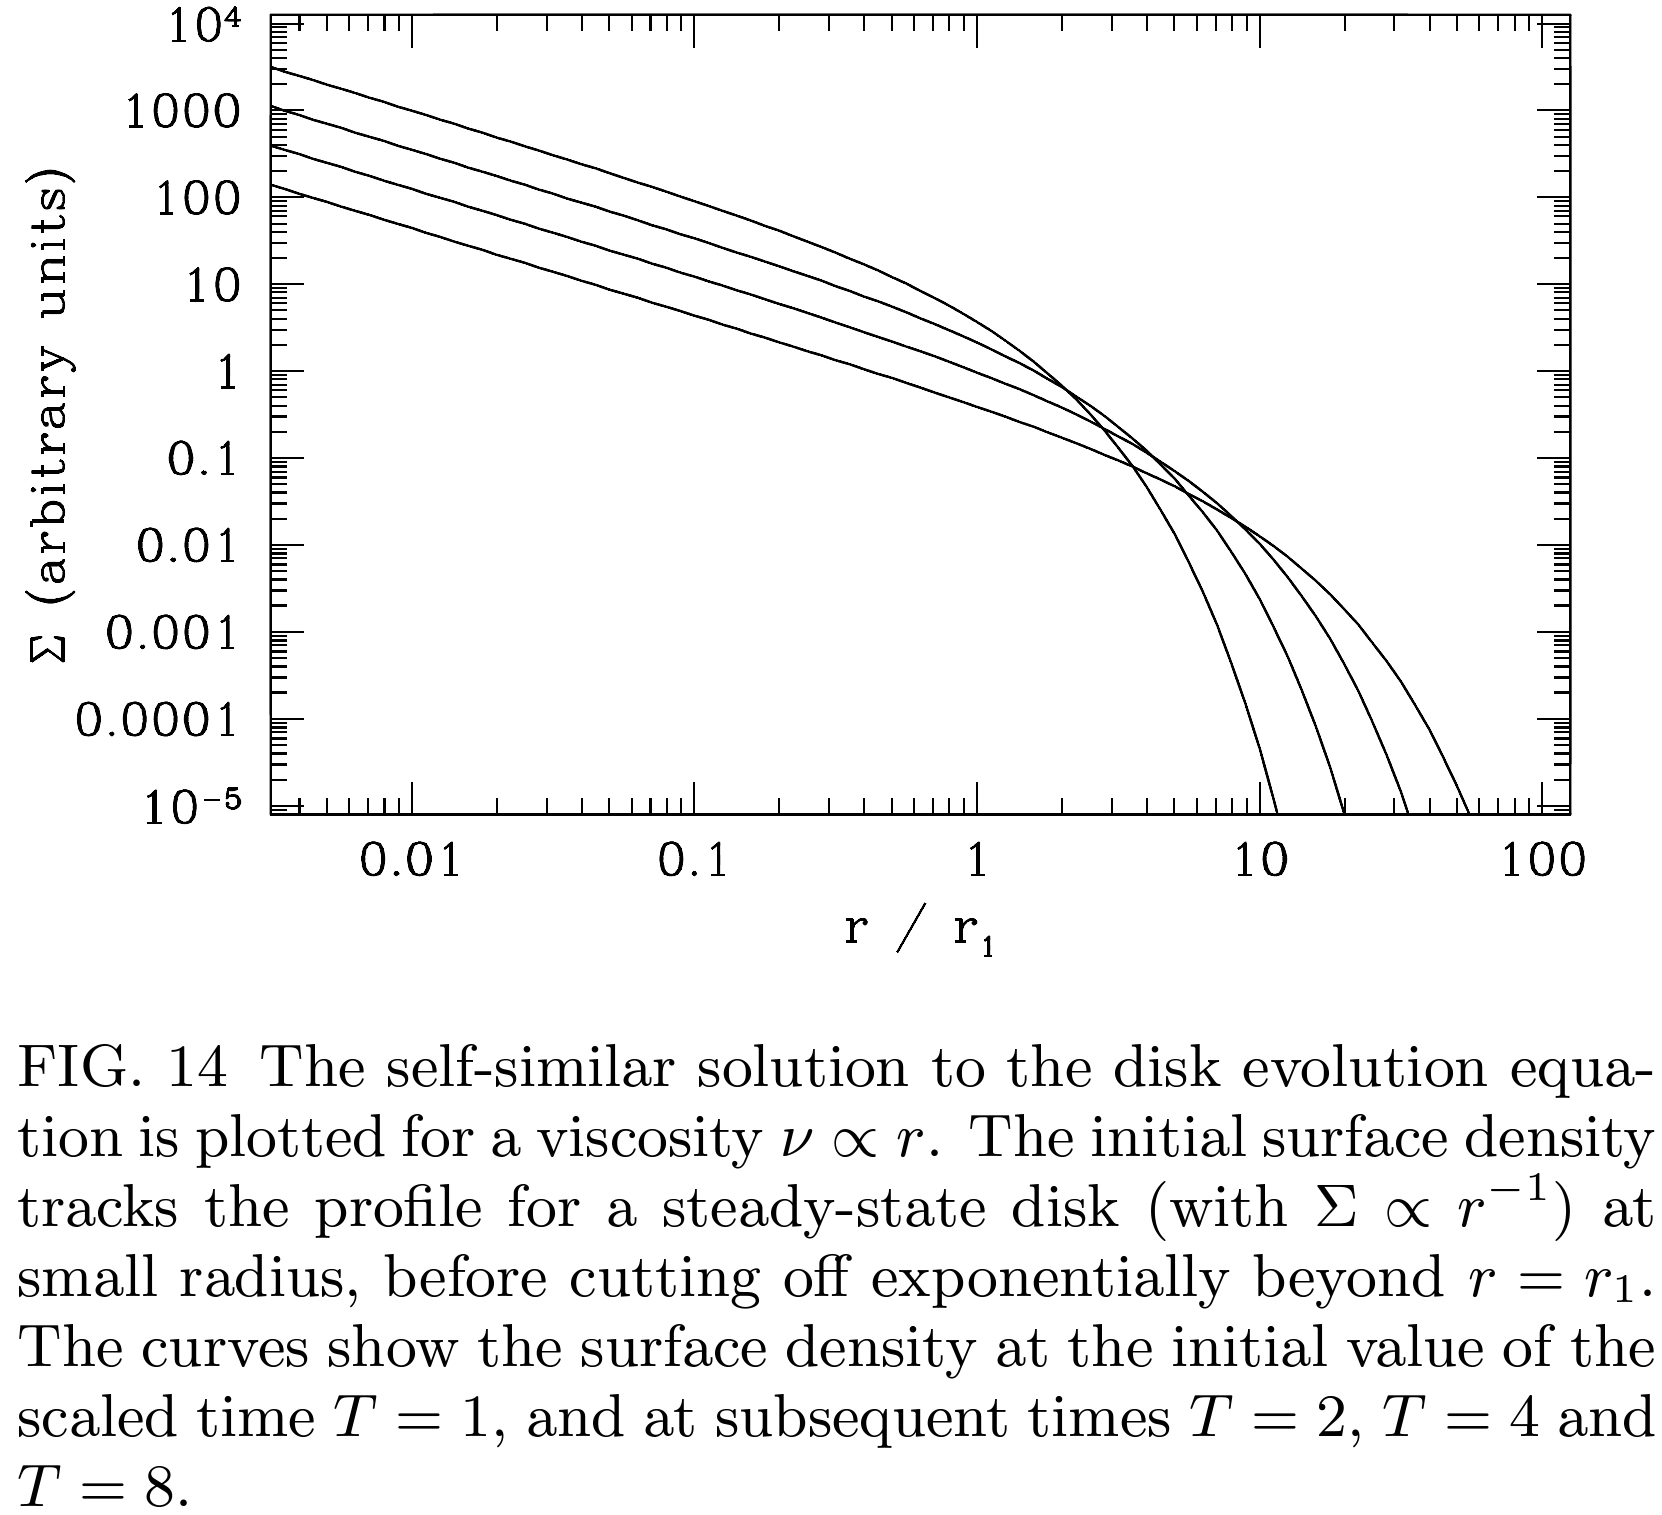
\includegraphics[trim={0cm 19cm 0 0},clip, keepaspectratio,width=0.48\textwidth]{selfsimilaralphadisk}
	\caption{Soluzione equazione \eqref{eq:sigmaevol} per $\nu\propto r\expy{\gamma}$ con $\gamma=1$. Da \cite{armitage2007lecture}.}\label{fig:selfsimilaralphadisk}
\end{wrapfigure}

Nei modelli di disco di accrescimento unidimensionali si parametrizza il trasporto di momento angolare ponendo
\begin{equation}
\nu=\alpha c_s H
\end{equation}
dove $\alpha$ \'e parametro da fissare, $c_s$ la velocit\'a del suono e H lo spessore del disco. Utilizzo l'equazione di conservazione della massa per riscrivere \eqref{eq:smoothedangularmomentumequation}:
\begin{equation}
\PDy{t}{\Sigma}=3\frac{1}{r}\PDof{r}[r\expy{1/2}\PDof{r}(\nu\Sigma r\expy{1/2})]\label{eq:sigmaevol}
\end{equation}

La struttura verticale \'e determinata dalla componente lungo z dell'attrazione del corpo centrale
%profilo termico determinato da equilibrio termico
\begin{equation}
\TDy{z}{P}=-\rho g_z=-\frac{GM_*}{r^2+z^2}\frac{z}{r}\rho=-\Omega^2\rho z
\end{equation}
mentre la struttura radiale del disco di gas \'e determinata dall'equilibrio idrostatico
\begin{equation}
\frac{v_g^2}{r}=\frac{GM_*}{r^2}+\frac{1}{\rho}\TDy{r}{P}
\end{equation}
dove ho introdotto $v_g$ velocit\'a a cui il gas orbita attorno alla stella centrale.

\begin{figure}[!ht]
	\begin{subfigure}[b]{0.39\textwidth}
		\centering
		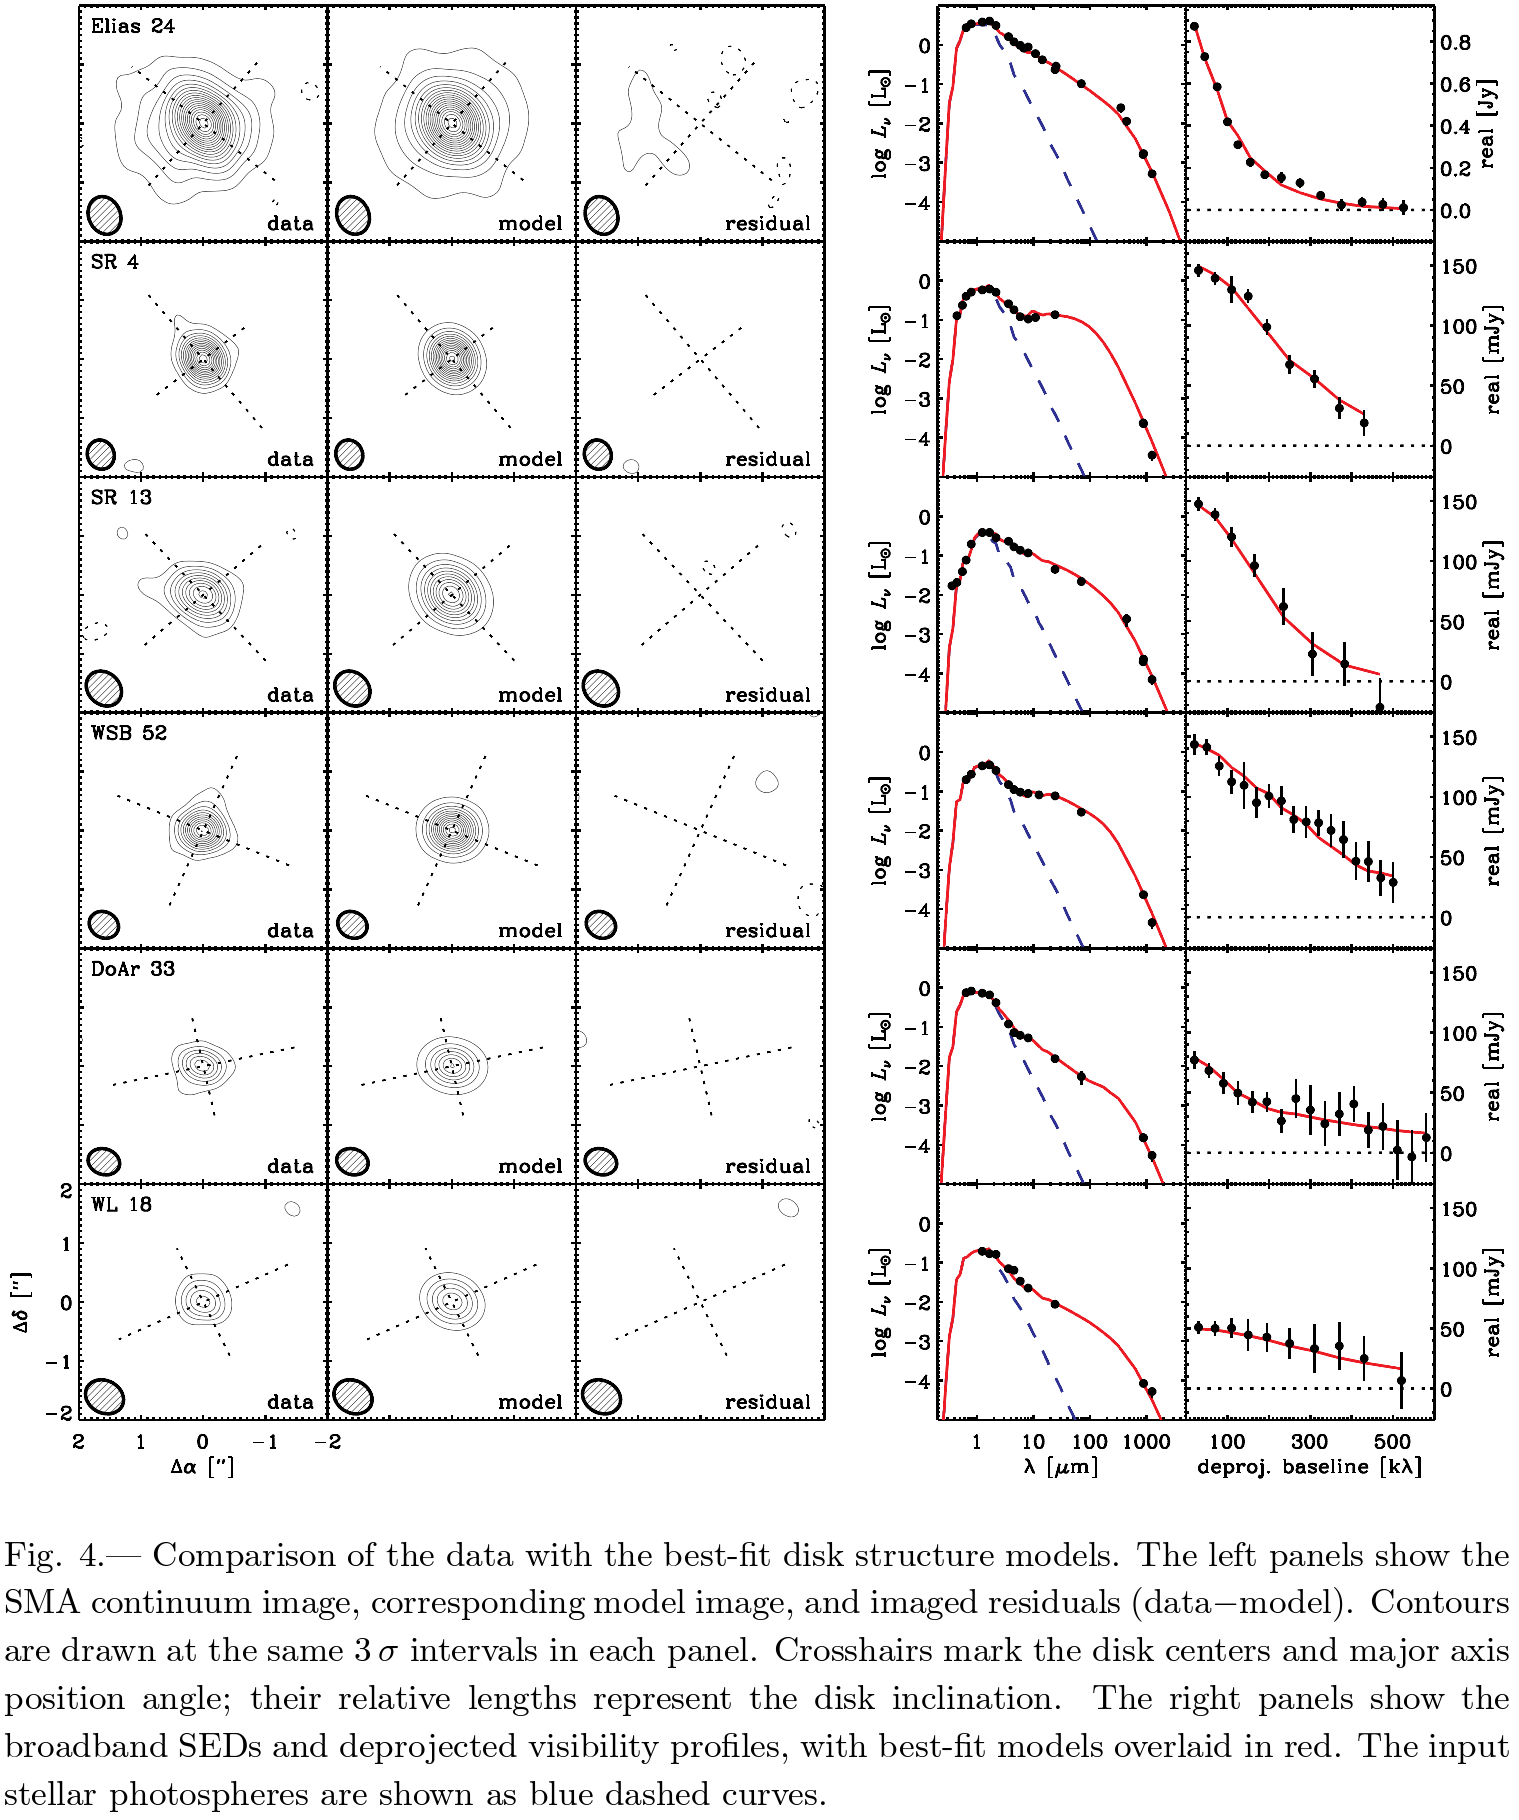
\includegraphics[trim={0cm 10cm 0 0},clip, keepaspectratio,width=0.98\textwidth]{SED-contours}
		\caption{Struttura dischi protoplanetari (flusso a $\lambda=\SI{880}{\micro\meter}$) e densit\'a spettrale. La linea tratteggiata viola indica la distribuzione di corpo nero della fotosfera stellare. Da \cite{andrews2010protoplanetary}.}\label{fig:SED-contours}
	\end{subfigure}
	~
	\begin{subfigure}[b]{0.55\textwidth}
		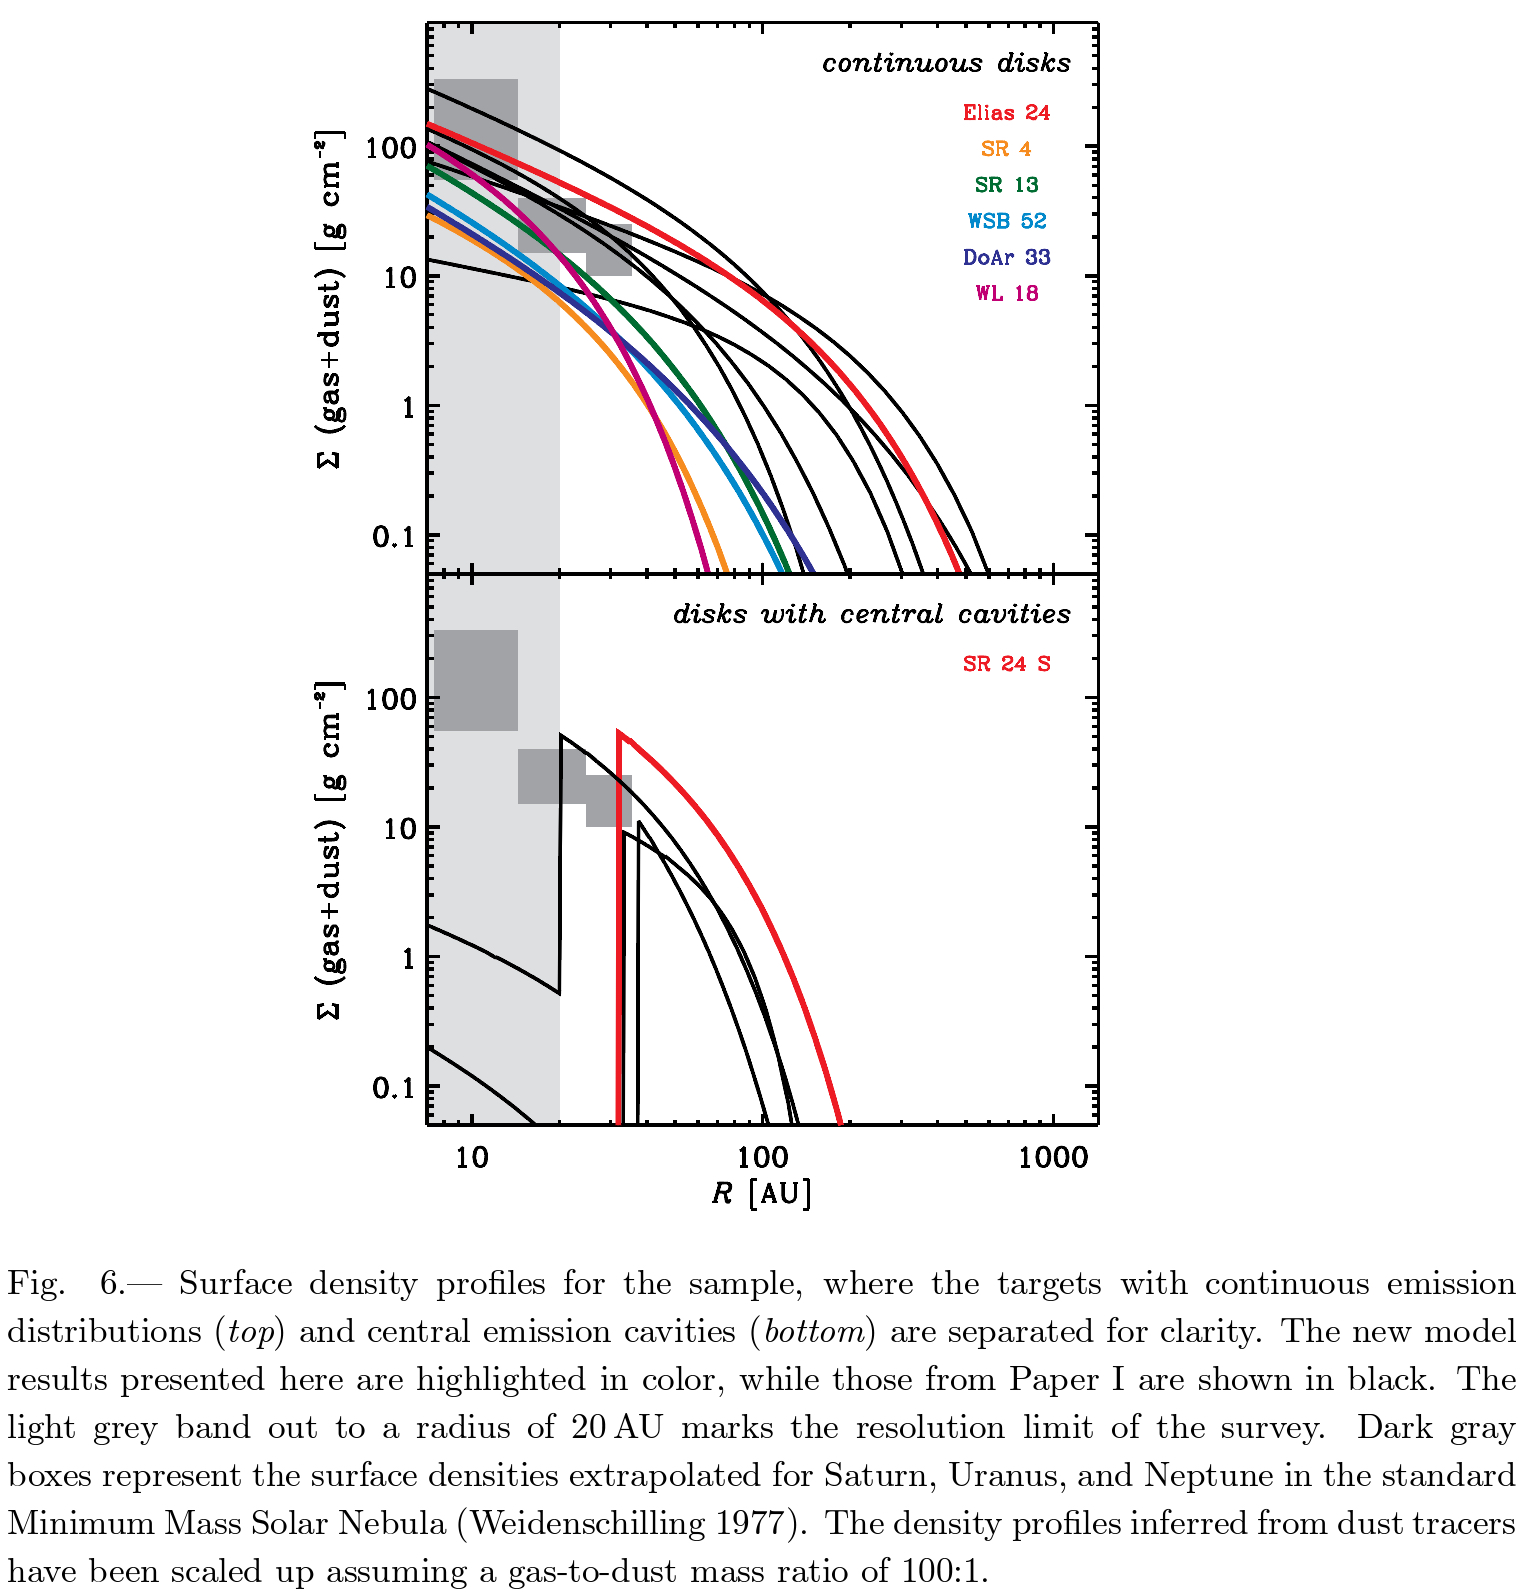
\includegraphics[trim={0cm 15cm 0 0},clip, keepaspectratio,width=0.98\textwidth]{diskdensity}
		\caption{Densit\'a superficiale dischi protoplanetari osservati nella regione di Ophiuchus ricavata risolvendo modello disco di accrescimento che riproduca densit\'a spettrale di energia osservata. I rettangoli grigi indicano densit\'a superficiale per la MMSN nella regione di Saturno, Urano e Nettuno. Da \cite{andrews2010protoplanetary}.}\label{fig:diskdensity}
	\end{subfigure}
\end{figure}

Attorno alle stelle giovani sovente si trovano strutture opache nel visibile ma otticamente sottili nelle onde infrarosse: risolvendo il modello di disco protoplanetario, avente come input la distribuzione della dimensione della polvere e rapporto gas/polvere, per riprodurre le caratteristiche spettrali e flusso termico osservati, note anche le caratteristiche della stella centrale, si determinano i parametri caratteristici del disco.

La figura (\subref{fig:SED-contours}) mostra le strutture attorno a stelle giovani del cluster Ophiuchus secondo profili di intensit\'a a \SI{880}{\micro\meter}. Se $\nu\propto r\expy{\gamma}$ una soluzione di \eqref{eq:sigmaevol} per $t=0$ \'e
\begin{equation}
\Sigma=(2-\gamma)\frac{M_d}{2\pi R_c^2}(\frac{r}{R_c})\expy{-\gamma}\Exp{-(\frac{r}{R_c})\expy{2-\gamma}}
\end{equation}
\cite{andrews2010protoplanetary} hanno osservato lo spettro emesso da oggetti nella regione di formazione stellare Ophiuchus determinando massa, dimensioni caratteristiche e viscosit\'a: $M_d=0.004-0.143\msun{}$, $\gamma=0.4-1.1$, $R_c=\SIrange{14}{198}{\astronomicalunit}$.

\begin{wrapfigure}[6]{l}{0.5\textwidth}
	\centering
	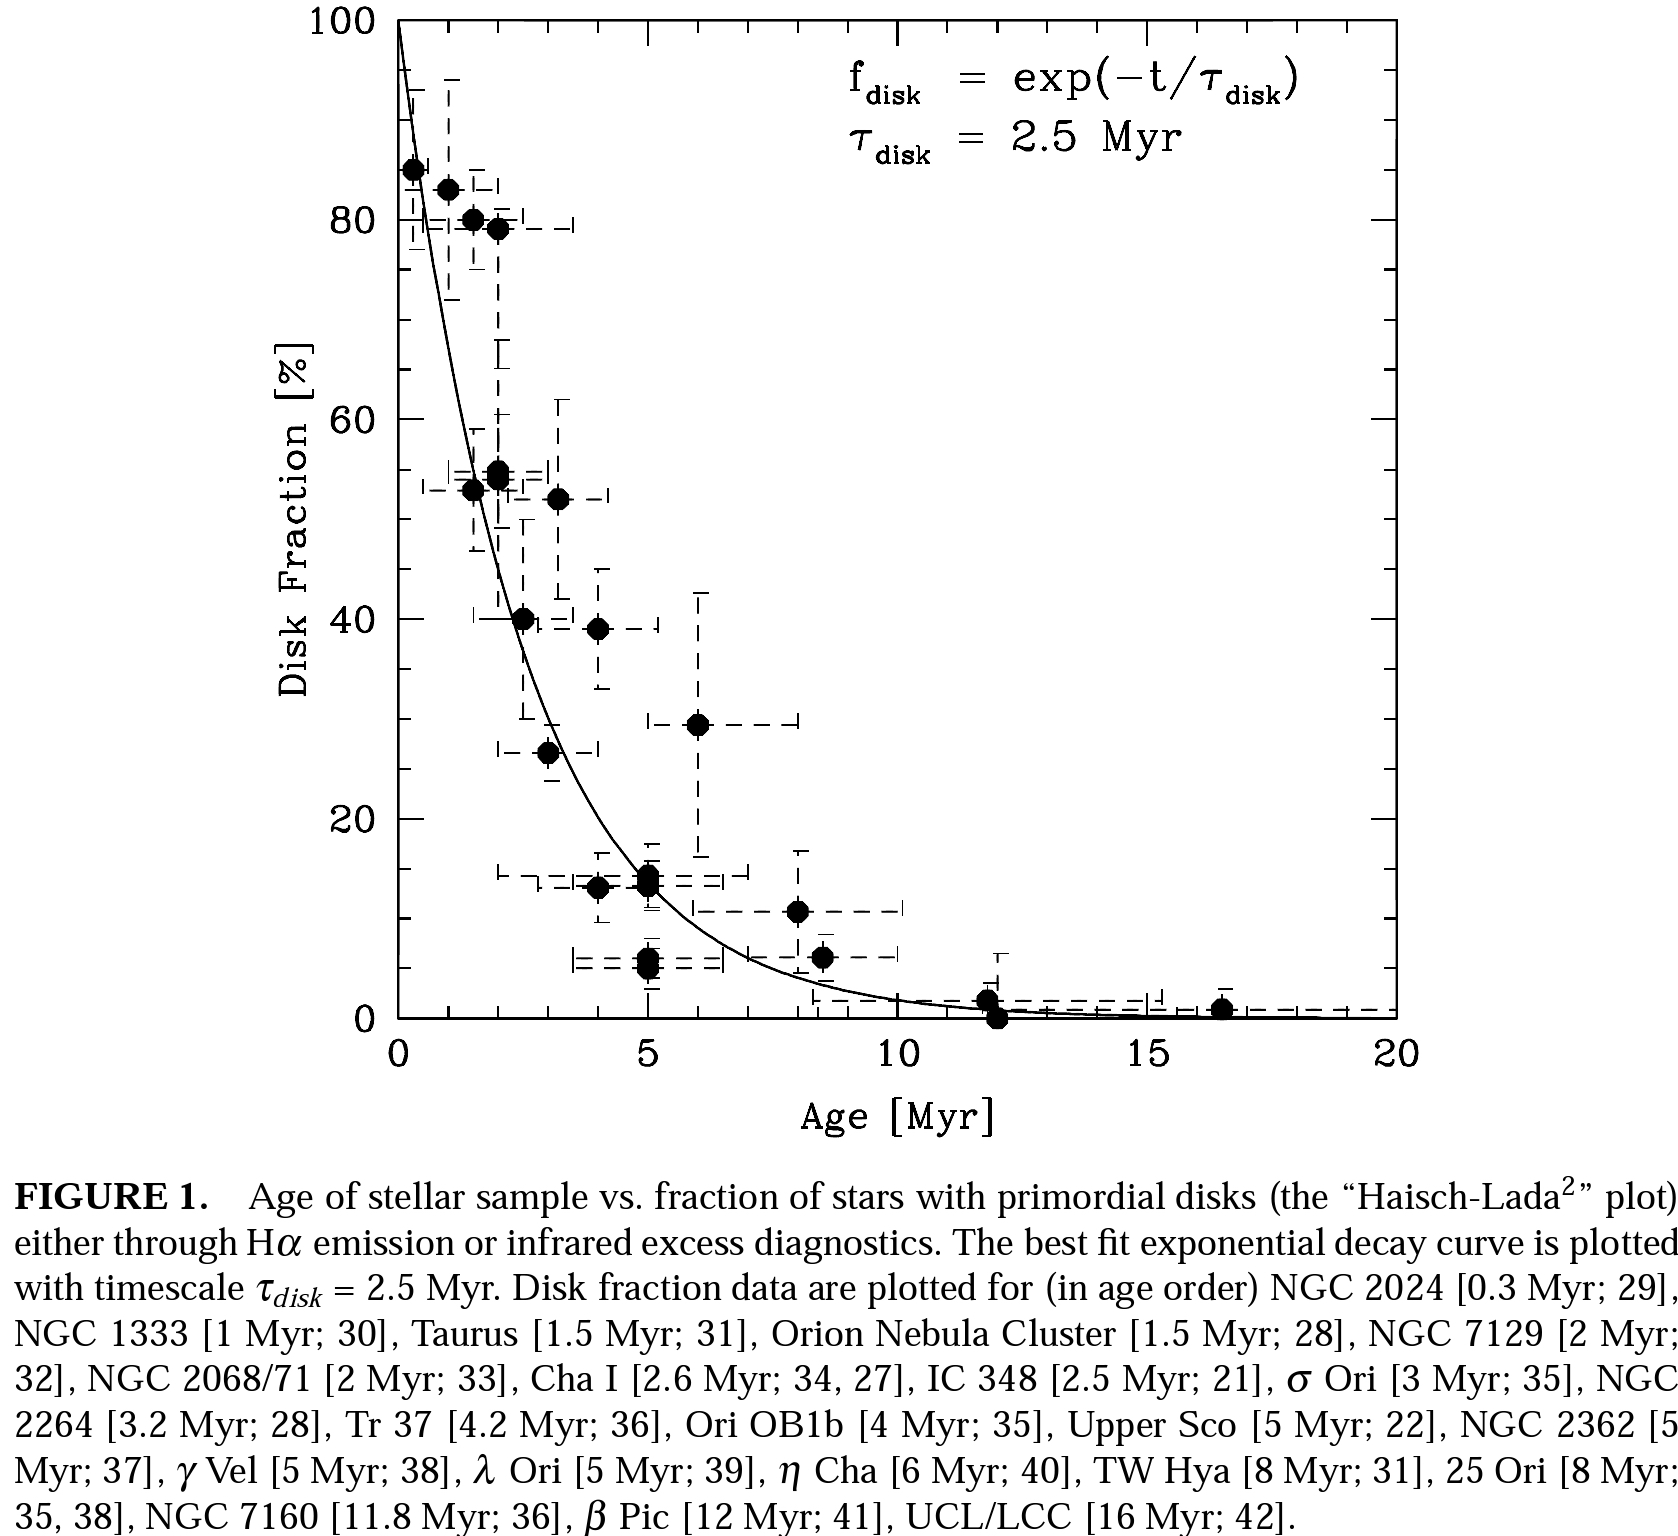
\includegraphics[trim={0cm 13cm 0 0},clip, width=0.49\textwidth,keepaspectratio]{clusterage-fstar}
	\caption{Frazione di stelle con disco protoplanetario in funzione dell'et\'a del cluster. Da \cite{mamajek2009initial}. }\label{fig:clusterage-fstar}
\end{wrapfigure}

In figura (\ref{fig:clusterage-fstar}) \'e riportata la frazione di stelle con dischi protoplanetari in funzione dell'et\'a del cluster. \'E possibile stimare tempo di vita caratteristico del disco considerando andamento esponenziale per frazione di dischi: secondo (\cite{mamajek2009initial}) $\tau_c\approx\SI{2.5}{\mega\year}$, mentre (\cite{haisch2001disk}) hanno determinato $\tau_c\approx\SI{6}{\mega\year}$.

\vspace{0.2\textheight}

\begin{workout}[Caratteristiche fittate proto-dischi]
	
\end{workout}

\begin{workout}[Profilo densit\'a verticale disco isotermo]
	Thin vertically isothermal disk
	\begin{align}
	&\rho(z)=\frac{\Sigma}{h\sqrt{2\pi}}\exp{-\frac{z^2}{2h^2}}
	&
	\end{align}
\end{workout}

\begin{workout}[Profilo termico del disco]
	
\end{workout}

\begin{workout}[Momento torcente in disco Kepleriano]
	\begin{align}
	&\sigma_{ij}=2\Sigma\nu D_{ij}=\Sigma\nu\begin{pmatrix}0&-\Omega\partial_r(r\Omega)\\-\Omega+\partial_r(r\Omega)&0
	\end{pmatrix}\\
	\end{align}
	Il momento torcente esercitato da S su $C^c$ \'e
	\begin{equation}
	T=\iint_{S^c}(\vec{r}\wedge\nabla\sigma)\,ds=\int_S\vec{r}\wedge(\sigma\,dl\vec{n})
	\end{equation}
	Nel caso S sia circonferenza di raggio r:
	\begin{equation}
	T_{\nu}=3\pi r^2\Omega_0\Sigma\nu
	\end{equation}
\end{workout}

\begin{workout}[Passive disks]
	(Refs: Ref: spectral energy distribution of T-Tauri star with passive circumstellar disk)
	Dust passively reirradiate star light
\end{workout}

\begin{workout}[Struttura verticale del disco, profilo termico]
	Pressione gas determinata da equilibrio idrostatico
\end{workout}

\begin{workout}[Viscous/turbulent disk]
	laminar (high momentum diffusion)
	mass inflow Gullbring98 \SIrange{e-9}{e-7}{\per\year}$\msun{}$
\end{workout}
\begin{workout}[MRI]
	fig 10.3:
	gammie 1996
\end{workout}

\begin{workout}[alpha prescription]
	$\vec{v}=(u_r,r\Omega)$, stress tensor $\sigma_{r\phi}=-\Sigma\exv{u_ru_{\phi}}$.
	Enhanced turbulent viscosity: $-\Sigma\exv{u_ru_{\phi}}=\Sigma\nu r\TDy{r}{\Omega}$, $\nu=v_TH$, $\alpha=v_T/c_s$
\end{workout}

\begin{workout}[Accretion disk sources]
	Lodato: classical disk physics
	o218, 296: disk formation, constrains from solar system
	the alpha disk pg 18: theory of turbulent accretion disk
\end{workout}

\begin{workout}[Isothermal cloud collapse!]
	
\end{workout}

\begin{workout}[Descrizione trasporto momento angolare tramite parametrizzazione viscosit\'a]
	Mass conservation + momentum conservation in viscous flow: angular momentum evolution. Phenomena: Shear viscosity - turbulence - MRI.
	Nei modelli 1D per disco di accrescimento si parametrizza viscosit\'a tramite $\nu=\frac{\eta}{\rho}\to\alpha c_s H$: la viscosit\'a molecolare \'e troppo bassa  per trasportare all'esterno il momento angolare sui tempi-scala osservati.
	Theory of turbulent accretion disk: pg 18, 8.
	Flusso di x-momentum lungo y $\rho\exv{u_xu_y}$, dove considero la velocit\'a dell'elemento di fluido $(v_x+u_x,u_y)$ dove le $u$ rappresentano fluttuazioni della velocit\'a: $\sigma_{xy}=-\rho\exv{u_xu_y}$.
	Ricordando la definizione di tensore degli stress e con $\vec{v}=v_x(y)\hat{x}$
	\begin{equation}
	\sigma_{ij}=\eta(\partial_jv_i+\partial_iv_j-\frac{2}{3}\delta_{ij}\partial_kv_k+\zeta\delta_{ij}\partial_kv_k \to \eta\TDy{y}{v_x}
	\end{equation}
	\begin{equation}
	\PDof{t}(\rho v_i)+\PDof{x_i}(\rho v_iv_j+T_{ij})=F_i
	\end{equation}
	Fluttuazioni: $\sigma_{ij}=-\rho\exv{u_iu_j}$.
	Viscosit\'a molecolare: $\exv{u_iu_j}=-\nu\TDy{x_j}{v_i}$.
	Turbulence: Reynpold stress $\tau_{ij}=-\rho\exv{v_jv_i}$, $\exv{u_iu_j}=-\nu_T\TDy{x_j}{v_i}$
	\begin{equation}
	\PDy{t}{\Sigma}=3\frac{1}{r}\PDof{r}[r\expy{1/2}\PDof{r}(\nu\Sigma r\expy{1/2})]
	\end{equation}
\end{workout}

\begin{workout}[Photoievaporation: X-EUV-FUV (Alexander13: The Dispersal of Protoplanetary Disks)]
	Protoplanetary disc evolution and dispersal: the implications of X-ray photoevaporation.
\end{workout}


\begin{workout}[Foto-evaporazione]
	(Photoevaporation: veras armitage 2003, Alexander13, Mordasini12. Internal/External).
	EUV($E\approx13.6eV$): ionization, FUV($E\approx6-13.6eV$): dissociation, X-ray
\end{workout}

\begin{workout}[classificazione YSO]
	section{YSO: distribuzione propriet\'a dischi protoplanetari}
	La classificazione empirica degli young stellar object (YSO) si basa sul valore di
	\begin{equation}
	\alpha_{IR}=\TDly{\lambda}{\lambda F_{\lambda}}
	\end{equation}
	tra \SIrange{2.2}{25}{\micro\meter}.
	\begin{itemize}
		\item Classe 0: Picco emissione in regione da lontano infrarosso a sub-millimetrica. Nubi molecolari compatte/protostelle.
		\item Classe 1: $\alpha_{IR}>0$ a \SI{2}{\micro\meter}. La stella accresce la maggior parte della sua massa finale.
		\item Classe 2: $0\geq\alpha_{IR}\geq-1.5$. Stella T-Tauri con disco otticamente spesso a $\lambda\leq\SI{10}{\micro\meter}$.
		\item Classe 3: $\alpha_{IR}\leq-1.5$. Stella T-Tauri con disco otticamente sottile a $\lambda\leq\SI{10}{\micro\meter}$.
	\end{itemize}
\end{workout}

\begin{workout}[Fit SED]
	Disk model
	\begin{align}
	\nu\propto R\expy{\gamma}\\
	\Sigma=(2-\gamma)\frac{M_d}{2\pi R_c^2}(\frac{R}{R_c})\expy{-\gamma}\\Exp{-(\frac{R}{R_c})\expy{2-\gamma}}
	\end{align}
\end{workout}


\begin{workout}[Initial conditionfor protostellar collapse]
	Andre 2000 - 
\end{workout}

\begin{workout}[T Tauri SED more flattish]
	Ref: spectral energy distribution of T-Tauri star with passive circumstellar disk
\end{workout}

\begin{workout}[physical processes in protoplanetary disk: IRexcess, accretion rate and lifetime,]
	(armitage 17): fig 1, accretion rate and lifetime (2.2 pg 5-6), inference from dust continuum (disk mass, evidence for mm-particle growth
	Le stelle giovani sono caratterizzate da eccesso infrarosso fra \SIrange{2.5}{10}{\micro\meter}:
	\begin{equation}
	\alpha_{IR}=\TDly{\nu}{\nu F_{\nu}}
	\end{equation}
	Sorgenti con SED declinante in mid infrared ($2.5-10\si{\micro\meter}$): $1.5<\alpha_{IR}=<0$. Active/passive: mass infall convert G into thermalradiation/reprocessed starlight.
	Refs: Perrymann 10.3 - disk formation pg 218 - 
	Classification based on slope of SED between $2-25\si{\micro\meter}$: $\alpha_{IR}=\TDly{\nu}{\nu F_{\nu}}=$ (Gail Hoppo 2010)
	Spitzer: forming regions within 500pc
	Formation: disk quickly forms as more distant material with high angular momentum, centrifugal radius $R(t)\propto\Omega^2 t^3$: . Class 0-I : protostellar disk, gravitational unstable (cloud collapse: the collapse of the cores of slowly rotating isothermal clouds, Terebey shu cassen 1984, selfsimilar collapse of isothermal spheres and star formation, shu 77). Singular isothermal sphere: $\rho=\frac{a^2}{2\pi G}r\expy{-2}$, $M(r)=\frac{2a^2}{G}r$.
\end{workout}

\begin{workout}[disco protoplanetario: distribuzioni condizioni iniziali]
	
	Initial disk mass
	(infall phase end, no more self-gravitational instabilities) - stability(shu90), MMSN hayashi81/weidenshilling77, observations(Andrews10,Manara16) points to $(0.1-10)\%$ stellar mass, distro log-normal with mean $0.01M_*$.
	
	{Disk lifetime}
	$1-10My$ with mean $3My$ (Haisch01, Mamajek09)
	
\end{workout}

\begin{workout}[YSO: classificazione ]
	SED: emissine a lunghezze d'onda millimetriche probano tutto il volume del disco, otticamente sottile a quelle lunghezze (Beckwith 90, Beckwith Sargent91).
	$S_{\nu}\propto B_{\nu}(1-\exp{-\tau})\approx B_{\nu}\tau$: emission produced near cold disk mid-plane.
	Rayleigh-jeans: $B_{\nu}\propto T$ and, since $\tau=\kappa\Sigma$, $S_{\nu}\propto \kappa\Sigma T$.
	(SED: Andrews williams 07)
	Survey: 0.3'', 345Ghz(870$\micro m$) 1Myr old Ophiuchus stars forming region
	The absolute chronology and thermal processing of solids in the solar protoplanetary disk (Connelly Ivanova 12)
\end{workout}

\begin{workout}[Selfsimilar initial disk density solution]
	Refs: Lynden-bel pringle 74
	Se la viscosit\'a \'e statica e distribuita secondo $\nu\propto r\expy{\gamma}$:
	\begin{align}
	&R_c=R_1\mathcal{T}\expy{1/(2-\gamma)}\\
	&M_d=M_{d,0}\mathcal{T}\expy{-1/2(2-\gamma)}\\
	\end{align}
\end{workout}

\begin{workout}[Analitic disk model]
	Chambers 09: On analytical model for the evolution of a viscous, irradiated disk
	On location of snowline in protoplanetary disk (lecar chiang 06)
	On the snow line in dusty PPD (Sasselov lecar 99)
	Accretion disks around young object I: Detailed vertical structure (D'alessio Lizzano 98)
\end{workout}

\begin{workout}[YSO properties distro]
	Refs: ''Protoplanetary Disk Structures in Ophiuchus''
	da dove sono ricavete nei PPS?
	mass: MMSN, andrews 10, manara 16
	lifetime: IR/UV excess: haisch 01, mamajek 09
	initial embryo starting position: relative spacing of few hill radii (kokubo ida 00), fill disk thinking of asyntituc isolation mass (Ida Lin 10), trapped (hasegawa pudritz 11, cridland 16)
	Hueso 05: evolution of protoplanetary disk, meyer 06 Formation and evolution of planetary systems, Udry 07: statistical properties of exoplanets)
	Distribuzione di probabilit\'a per condizioni iniziali.
	
	Initial condition for planet formation (protoplanetry disk \cite{meyer2006formation}): disk metallicity, mass, lifetime, \ldots
	
	{Metallicity and Dust/Gas}
	$[M/H]$ distro modelled as normal: $\mu=-0.02$, $\sigma=0.22$ (photosphere of solar-like stars in solar neighborhood): Santos05.
	$f_{dg}=f_{dg,\odot}10\expy{[M/H]}$ with $f_{dg,\odot}=0.01-0.02$.
\end{workout}

\begin{workout}[Classificazione YSO: convenzioni]
	Sorgenti con SED declinante in mid infrared ($2.5-10\si{\micro\meter}$): $1.5<\alpha_{IR}=<0$. Active/passive: mass infall convert G into thermalradiation/reprocessed starlight.
	Refs: Perrymann 10.3 - disk formation pg 218 - 
	Classification based on slope of SED between $2-25\si{\micro\meter}$: $\alpha_{IR}=\TDly{\nu}{\nu F_{\nu}}=$ (Gail Hoppo 2010)
	Spitzer: forming regions within 500pc
	Formation: disk quickly forms as more distant material with high angular momentum, centrifugal radius $R(t)\propto\Omega^2 t^3$: . Class 0-I : protostellar disk, gravitational unstable (cloud collapse: the collapse of the cores of slowly rotating isothermal clouds, Terebey shu cassen 1984, selfsimilar collapse of isothermal spheres and star formation, shu 77). Singular isothermal sphere: $\rho=\frac{a^2}{2\pi G}r\expy{-2}$, $M(r)=\frac{2a^2}{G}r$
\end{workout}

\begin{workout}[Refs dischi protoplanetari]
	Ciesla Dullemond10 
	Perryman ch 10
	williams cieza 11
	Andrews 09-10
	mamajek 2009 - Initial conditions of planet formation: lifetimes of primordial disks
	infrared excess: gail hoppe10
\end{workout}

{\let\clearpage\relax\let\cleardoublepage\relax
\chapter{Caratteristiche della popolazione di esopianeti}
}

\begin{wrapfigure}[10]{l}{0.65\textwidth}
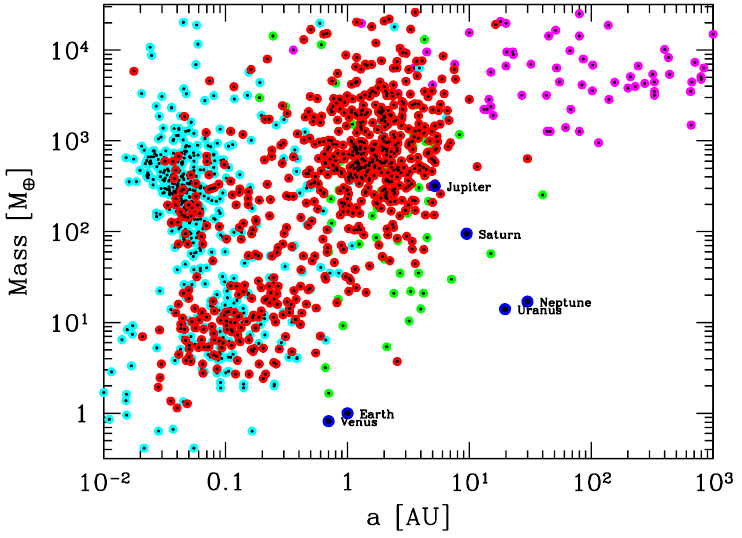
\includegraphics[trim={0cm 0 0 0},clip, width=0.65\textwidth]{obsMa}
\caption{Diagramma massa-distanza degli esopianeti in ''The extrasolar planet encyclopedia''. Rosso, celeste, magenta e verde sono pianeti rivelati tramite RV, T, osservazione diretta e microlensing. Da \cite{mordasini2018planetary}.}\label{fig:Maplot}
\end{wrapfigure}

\begin{workout}[bias osservativi tecnica/strumento]
La popolazione degli esopianeti osservata riflette quella reale tramite gli effetti di selezione dovuti alla probabilit\'a di rivelamento della tecnica/strumento particolari.
\end{workout}

Le osservazioni pi\'u numerose sono basate sull'osservazione della velocit\'a lungo la linea di vista dovuto al moto della stella attorno al baricentro del sistema stella pianeta (RV) o differenza nella luminosit\'a dovuto al transito del pianeta tra stella e osservatore (T). \'E evidente da \ref{fig:Maplot} che i pianeti extra-solari osservati riempono una vasta regione del diagramma $(a,M)$.

\begin{workout}[bimodal radius distro is observed by transit?]
Characterization of exoplanets from their formation II. The planetary mass-radius relationship pg 21: bimodal radius distribution
\end{workout}

\begin{workout}[frequenza sistemi planetarii:doppler + transito]
tab.1 mayor11(RV)
tab.1: occurrence and architecture exoplanetary system 
\end{workout}

\begin{workout}[Occurence rate]
\begin{itemize}
\item Coralie hot jupiter: giant planets $M\sin{i}>0.2\mjupiter$ and $a<0.1au$; $5.6\%$ giant out to 4au
\item Lick/Keck/AAT ($M\sin{i}>0.5\mjupiter$): $1.2\%$ stars have hot jupiter and $6.6\%$ giant within 5 au
\item ...
\end{itemize}
\end{workout}

\vspace{5cm}

\section{Popolazione esopianeti rilevati tramite RV}

Considero il moto stellare attorno al centro di massa del sistem stella pianeta:
se l'asse z \'e lungo la linea di vista la posizione della stella \'e $z=r(t)\sin{i}\sin{(\omega+\nu)}$ e per la velocit\'a radiale:
\begin{equation}
v_r=\dot{z}=K[\cos{(\omega+\nu)}+e\cos{\omega}]\label{eq:vrsignal}
\end{equation}
\begin{equation}
K=\frac{2\pi}{P}\frac{a_*\sin{i}}{(1-e^2)\expy{1/2}}=(\frac{2\pi G}{P})\expy{1/3}\frac{M_p\sin{i}}{(M_p+M_*)\expy{2/3}}\frac{1}{(1-e^2)\expy{1/2}}
\end{equation}
dove $K$ \'e la semi-ampiezza.
Numero misure della velocit\'a radiale permettono di determinare alcuni parametri orbitali ($e$, $P$, $t_p$, $\omega$) e la massa minima $M_p\sin{i}$.

\begin{errata}[Detection probability]
Per probabilit\'a di rivelamento del $50\%$ la minima massa planetaria \'e
\begin{equation}
M_{p,min}\approx4\mearth{}(\frac{N}{20})\expy{-1/2}(\frac{\sigma}{\SI{1}{\meter\per\second}})(\frac{P}{\SI{1}{\day}})\expy{1/3}(\frac{M_*}{\msun{}})\expy{2/3}
\end{equation}
dove $\sigma$ tiene conto errori strumentali e rumore stellare.
\end{errata}
Per sistemi multipli consideriamo la sovrapposizione lineare di $n_p$ termini \eqref{eq:vrsignal}: viene sottratto il segnale Kepleriano dominante fino a che resta solo rumore.

%Detection probability cumming 2004
La probabilit\'a di rivelamento \'e determinata dall'ampiezza del moto radiale della stella attorno al centro di massa K, il rumore strumentale e stellare, la durata dell'osservazione e la forma dell'orbita.

\begin{figure}[!ht]
\centering
\begin{subfigure}[b]{0.4\textwidth}
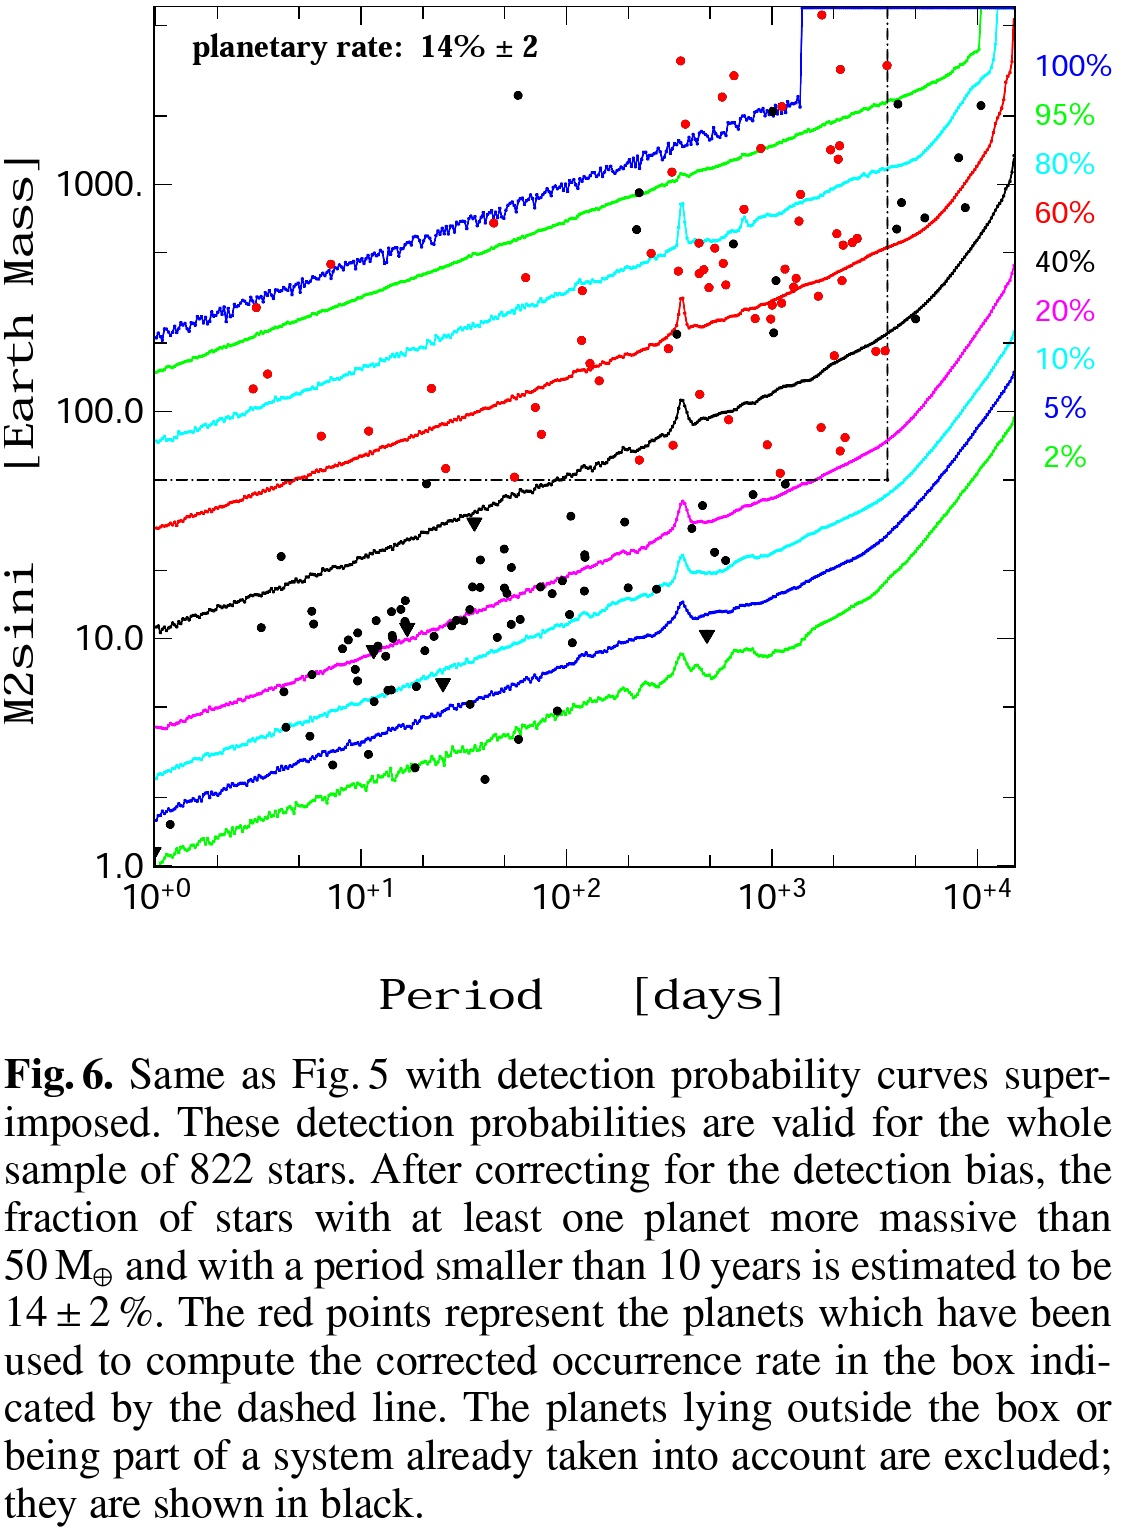
\includegraphics[trim={0cm 17cm 1cm 0},clip, width=0.99\textwidth]{PMfreq-e23}\label{fig:PMfreq-e23}
\end{subfigure}
~
\begin{subfigure}[b]{0.4\textwidth}
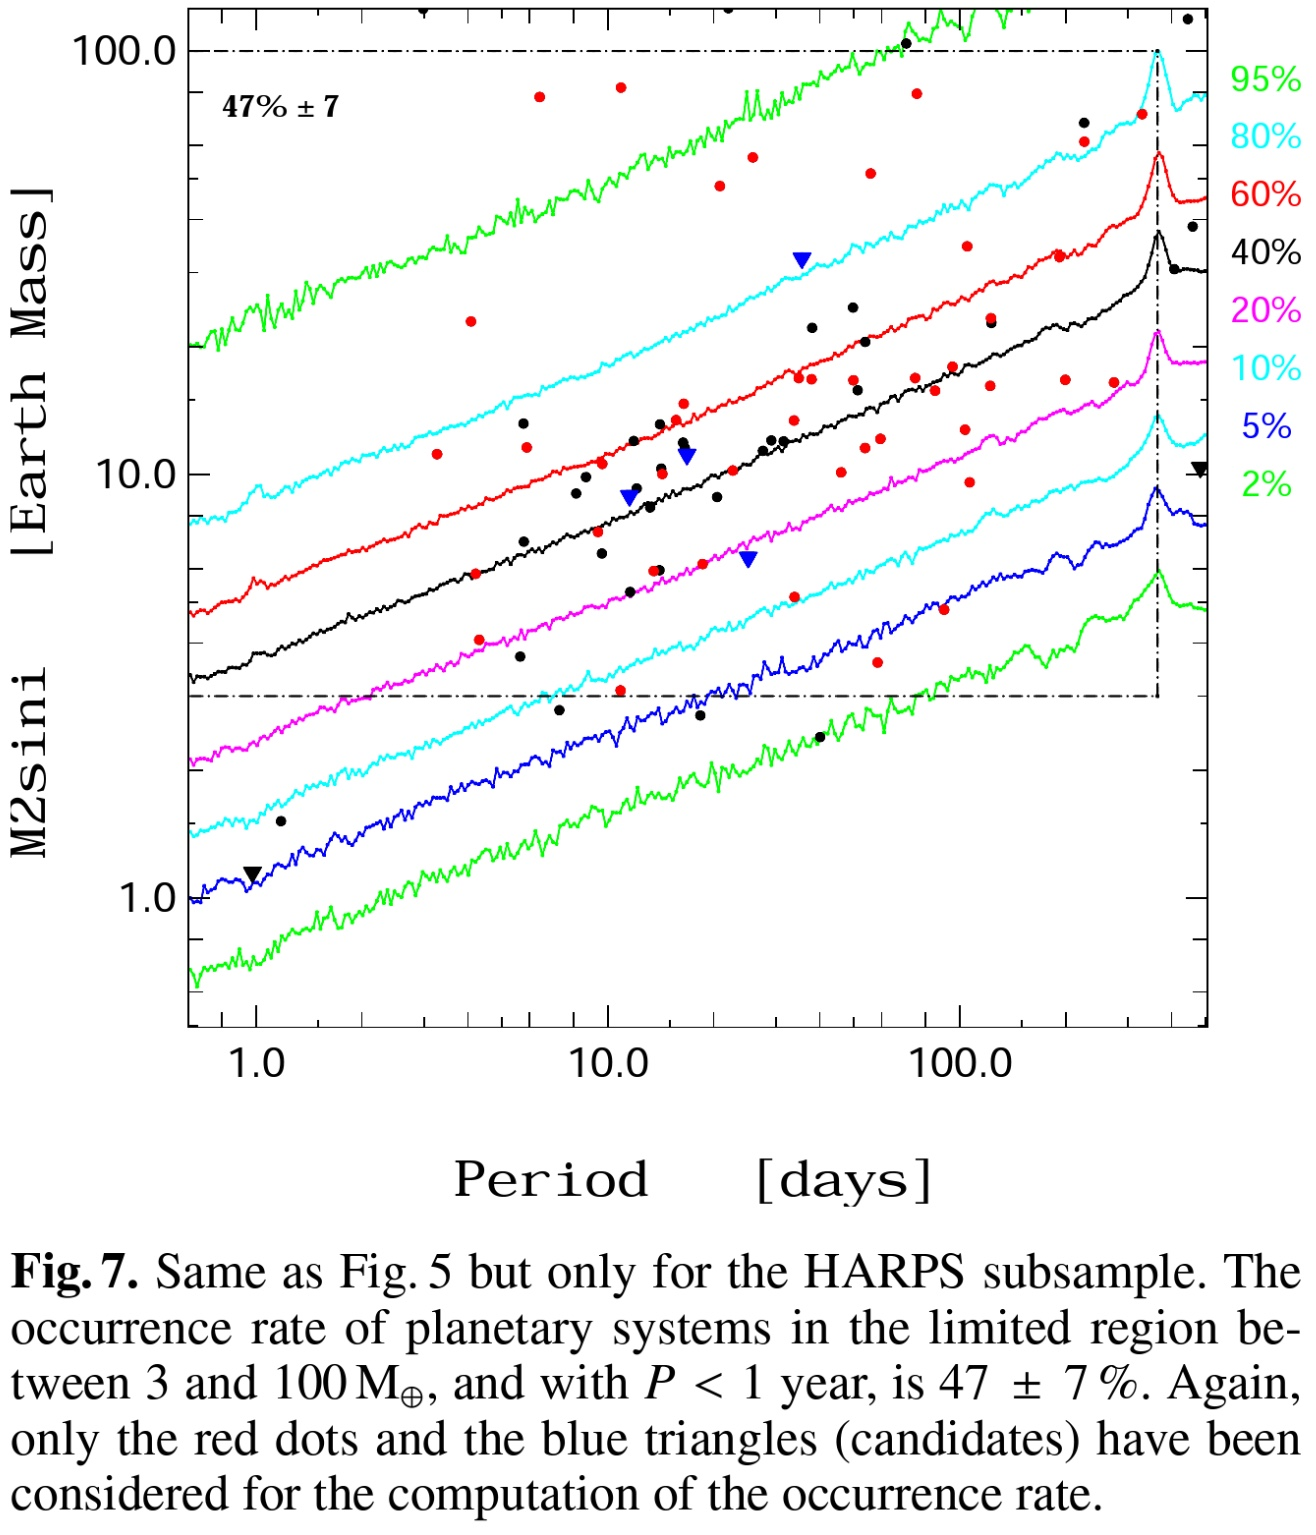
\includegraphics[trim={0cm 10cm 0 0},clip, width=0.99\textwidth]{PMfreq-e12}\label{fig:PMfreq-e12}
\end{subfigure}%

\begin{subfigure}[b]{0.4\textwidth}
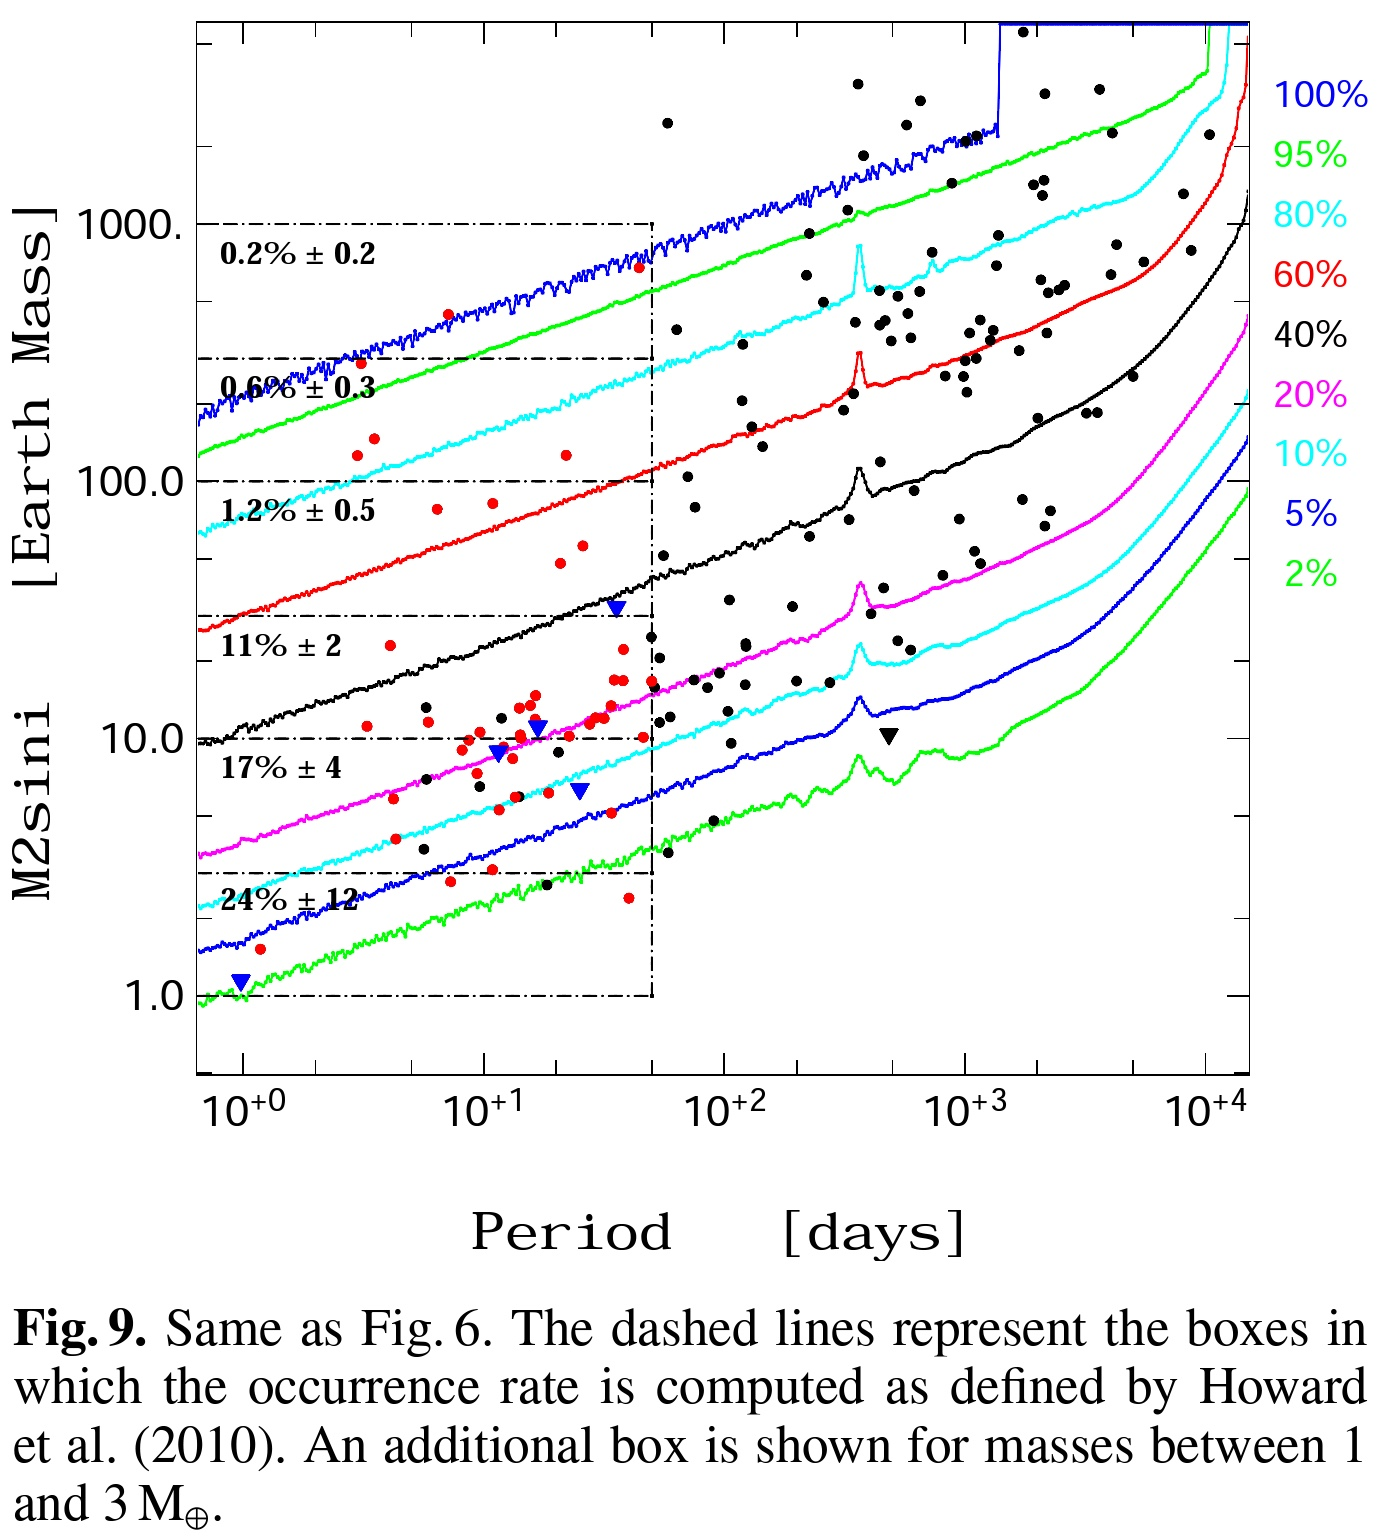
\includegraphics[trim={0cm 8cm 0 0},clip, width=0.99\textwidth]{PMfreq-short}\label{fig:PMfreq-short}
\end{subfigure}
\caption{Diagramma massa-periodo: frazione di stelle che ospitano pianeta con caratteristiche nella regione evidenziata. Da sinistra a destra: $P<10\si{\year}$ e $M>50\mearth{}$, $P<1\si{\year}$ e $M>3-100\mearth{}$, $P<50\si{\day}$ e $M=1-3/3-10/10-30/30-100/100-300/300-1000$. Da \cite{mayor2011harps}.}\label{fig:PMfreqs}
\end{figure}

\begin{workout}[HARPS low activity stars sample]
mayor 11 fig 1
\end{workout}

I tre diagrammi (\ref{fig:PMfreqs}) mostrano la frequenza dei pianeti in delimitate regioni del diagramma periodo-massa ($P-M$)  ricavate da \cite{mayor2011harps} determinata utilizzando un sottocampione di stelle per cui la probabilit\'a di rivelazione relativa alla regione del diagramma $(P-M)$ \'e $99\%$: accanto alle linee continue nei diagrammi $(P,M)$ sono indkicate le percentuali di stelle per cui \'e possibile ottenere una probabilit\'a di rivelamento del $99\%$ nella parta inferiore del diagramma.

\begin{figure}[!ht]
\begin{subfigure}[b]{0.49\textwidth} \centering 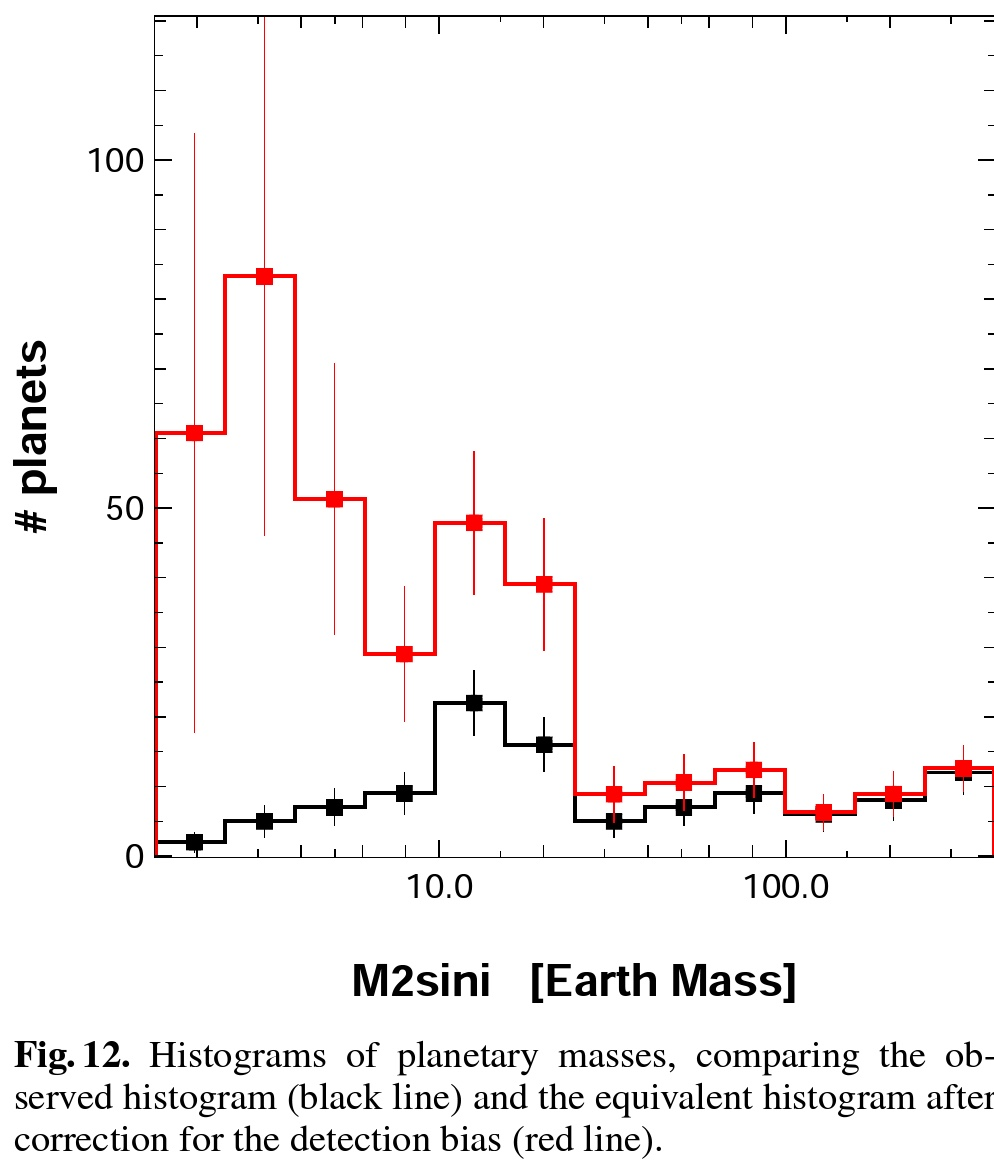
\includegraphics[trim={0cm 5cm 0 0},clip, width=0.94\textwidth]{freqvsM}
\caption{Distribuzione di massa di massa dei pianeti: in rosso distribuzione corretta per bias osservativi. Da \cite{mayor2011harps}.}\label{fig:freqvsM} \end{subfigure}
~
\begin{subfigure}[b]{0.49\textwidth} \centering 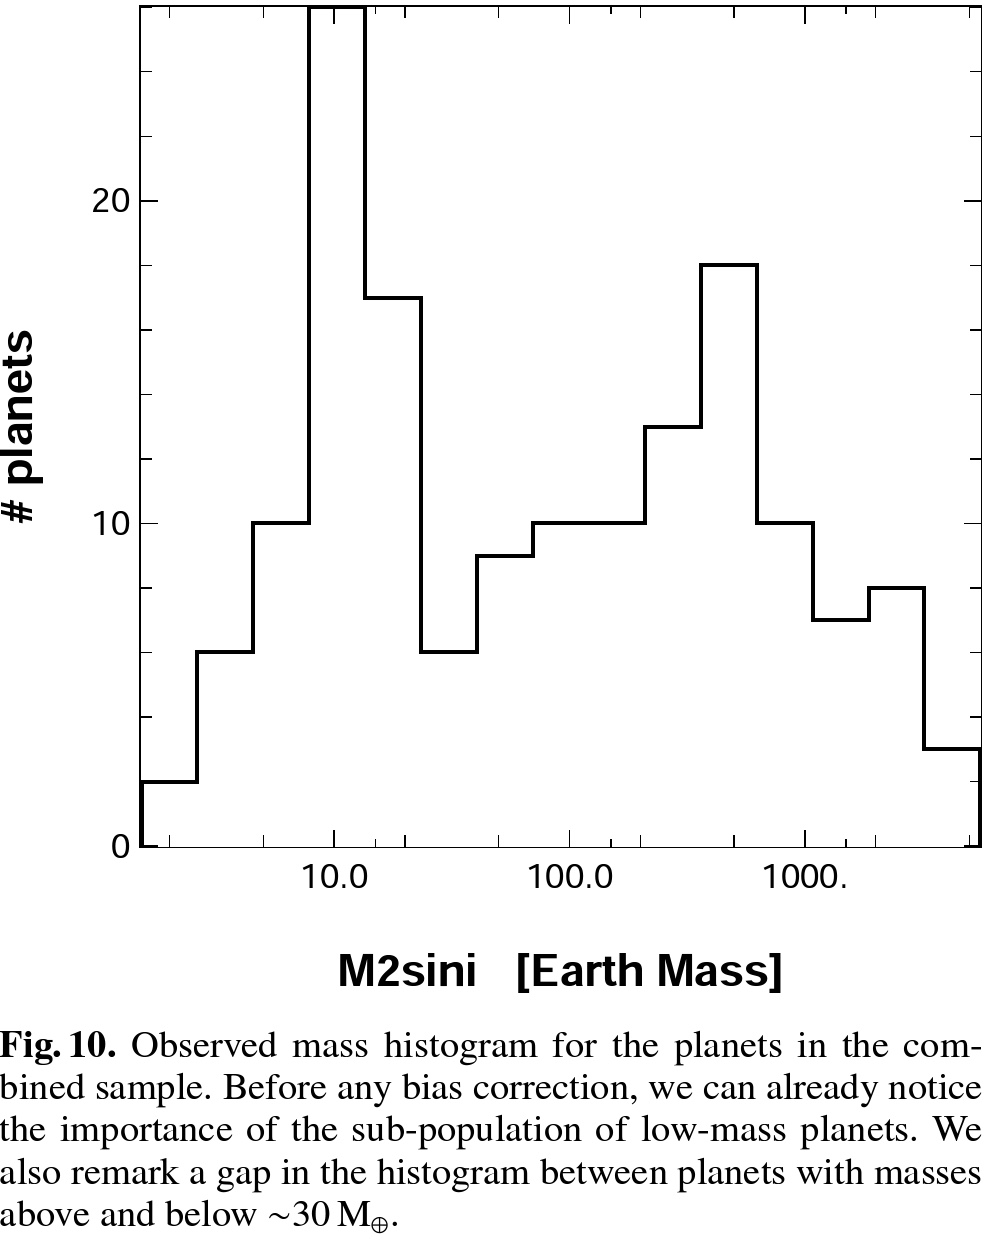
\includegraphics[trim={0cm 8cm 0 0},clip, width=0.94\textwidth]{freqvsMcomb}
\caption{Distribuzione di massa dei pianeti osservata. Da \cite{mayor2011harps}.}\label{fig:freqvsMcomb}
\end{subfigure}
\end{figure}

\begin{figure}[!ht]
\centering 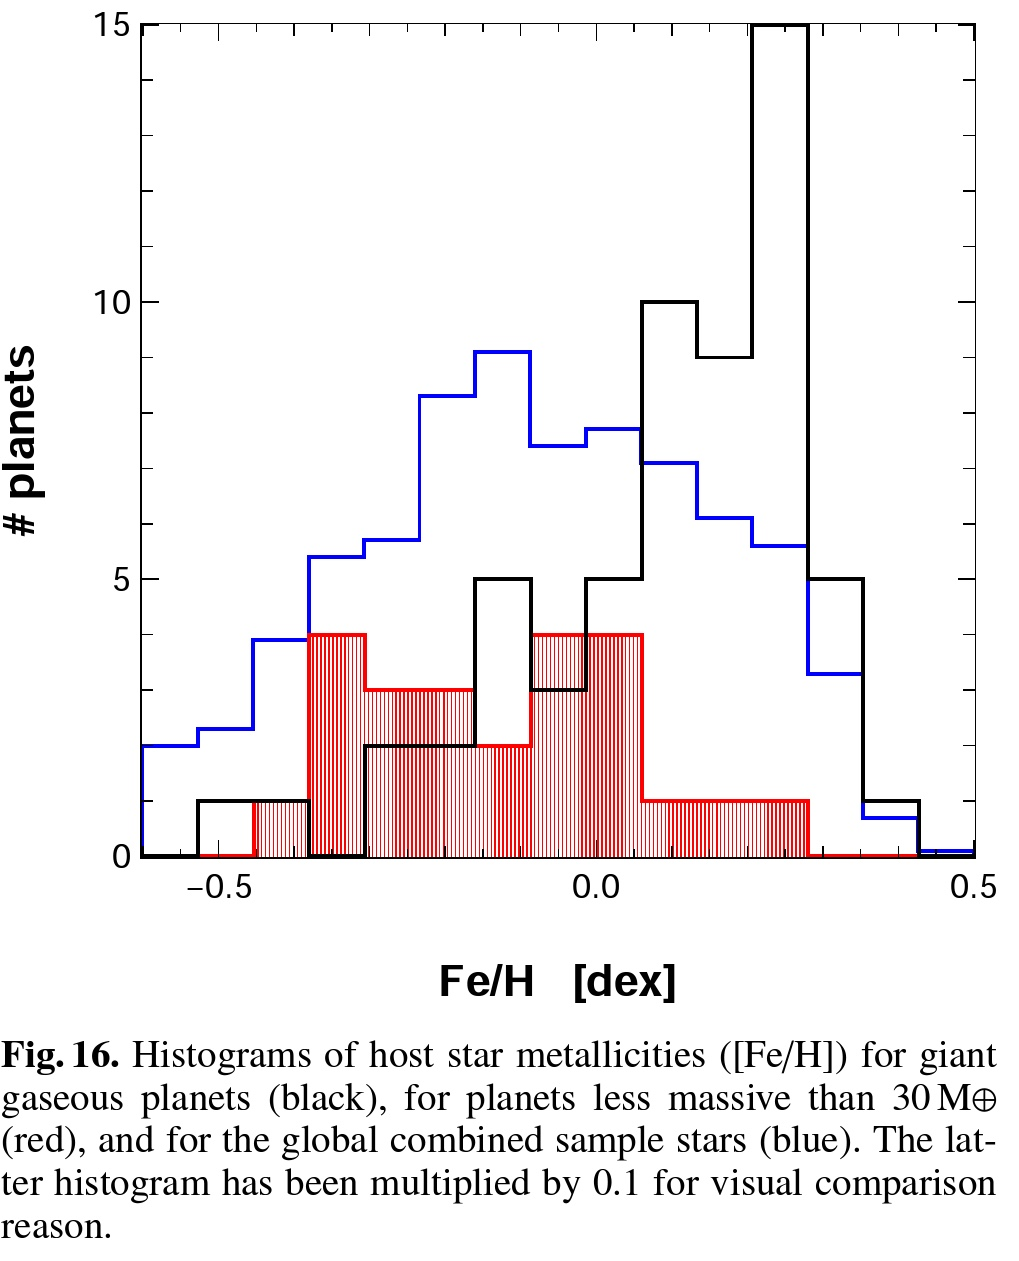
\includegraphics[trim={0cm 8cm 0 0},clip, width=0.43\textwidth]{PfreqvsFeH}
\caption{Numero di pianeti in funzione della metallicit\'a stellare: nero dei giganti gassosi, rosso dei pianeti con $M\leq30\mearth{}$ e blu combinata. Da \cite{mayor2011harps}.}\label{fig:PfreqvsFeH}
\end{figure}

La distribuzione di massa (figure \subref{fig:freqvsM}, \subref{fig:freqvsMcomb}) mostra un'abbondante popolazione di pianeti di massa piccola e una rapida diminuzione attorno a $10\mearth{}$; la distribuzione dei periodi mostra aumento dei pianeti giganti ($M>30\mearth{}$) a maggiore periodo orbitale (figura \subref{fig:freqvsPgiant}) e concentrazione pianeti piccola massa a $P=10-100\si{\day}$ (figura \subref{fig:freqvsPlowM}).

La figura \ref{fig:PfreqvsFeH} mostra l'assenza di correlazione tra la metallicit\'a della stella e la frequenza di pianeti di piccola massa fino a $30-40\mearth{}$ al contrario di quello che accade per pianeti giganti.

\begin{figure}[!ht]
\begin{subfigure}[b]{0.49\textwidth} \centering 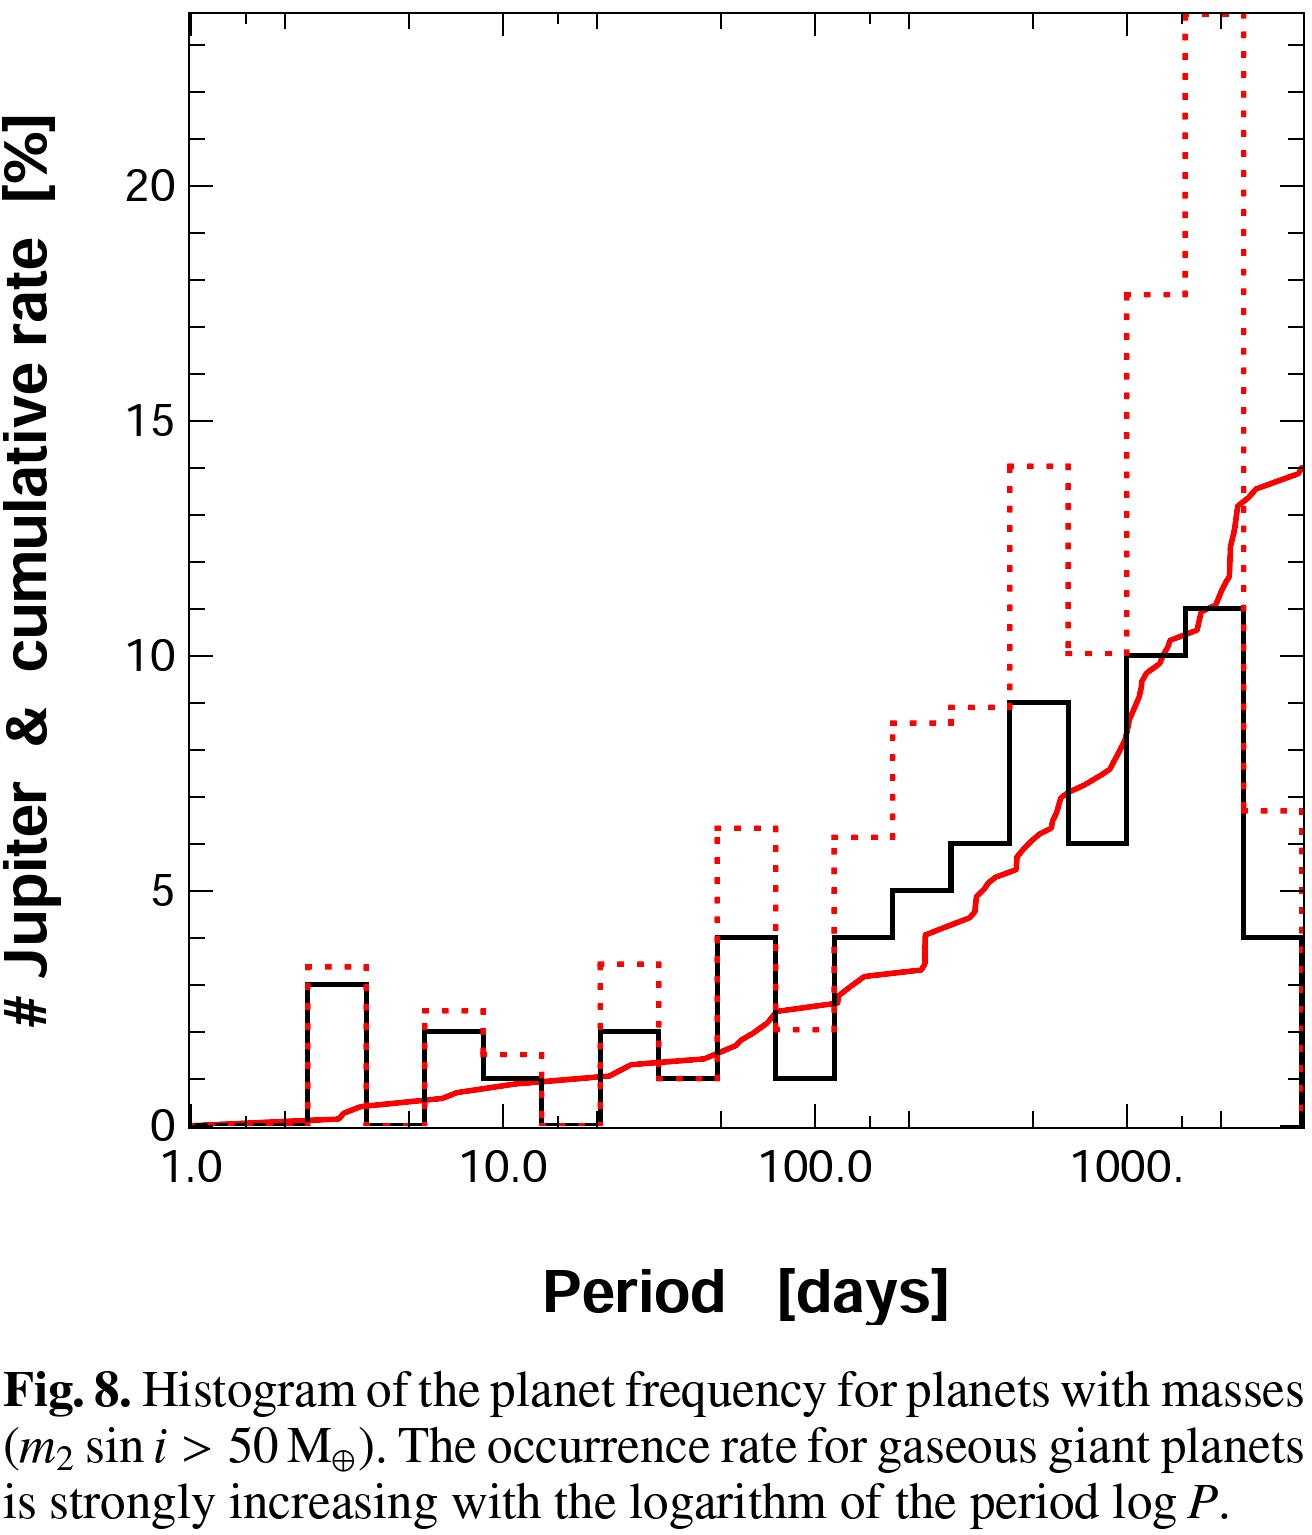
\includegraphics[trim={0cm 6cm 0 0},clip, width=0.98\textwidth]{freqvsPgiant}\caption{Frequenza pianeti con $M\geq 30\mearth{}$ in funzione del periodo orbitale; in rosso  tratteggiato con correzione bias osservativi. Da \cite{mayor2011harps}.}\label{fig:freqvsPgiant} \end{subfigure}
~
\begin{subfigure}[b]{0.49\textwidth} \centering 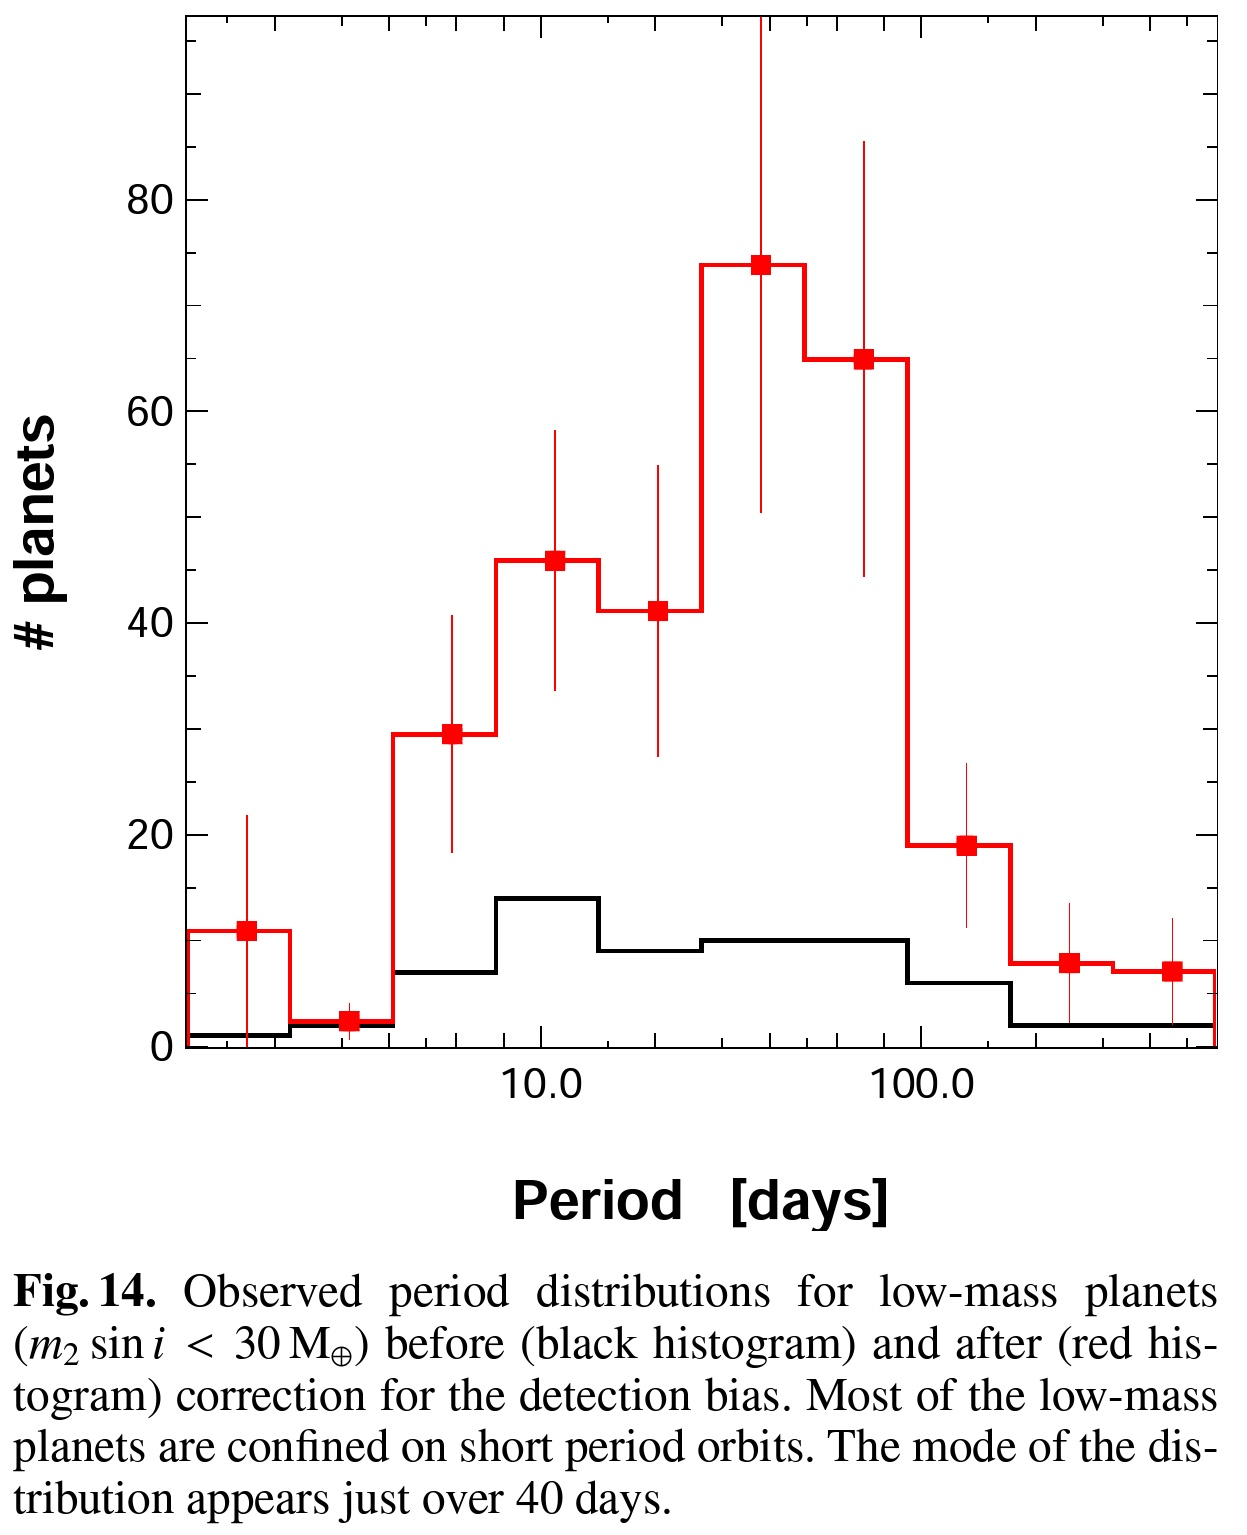
\includegraphics[trim={0cm 10cm 0 0},clip,width=0.98\textwidth]{freqvsPlowM} \caption{Frequenza pianeti con $M\leq 30\mearth{}$ in funzione del periodo orbitale; in rosso con correzione bias osservativi. Da \cite{mayor2011harps}.}\label{fig:freqvsPlowM}
\end{subfigure}
\end{figure}

\begin{workout}[Spostamento picco superterre-aumento massa pianeti giganti all'aumentare del periodo]
Una comprensione pi\'u ampia si ha studiando la distribuzione dei pianeti nel diagramma massa-periodo (M-P): elenco alcune caratteristiche della distribuzione dei pianeti osservati (da \cite{mayor2011harps}).
\begin{itemize}
\item Il picco della densit\'a di super-terre si sposta da $6\mearth{}$ a $10\mearth{}$ per periodi da \SI{10}{\day} a \SI{100}{day}
%\item Non sono osservati pianeti fino a $50\mearth{}$ con $P>\SI{1000}{\day}$
\item il pianeta gassoso pi\'u massiccio aumenta da $1\mjupiter{}$ a $15\mjupiter{}$ passando da $P\approx\SI{1}{\day}$ a $P\approx\SI{15}{\year}$.
\end{itemize}
\end{workout}


\begin{workout}[Origin of metallicity excess: stellar structure]
Pinsonneault depoy caffee 01
\end{workout}•

\begin{workout}[minimo in mass distro]
\'e un minimo? ha un significato?
\end{workout}

\begin{workout}[dtectability and selection effects (pg 14)]
Perrymann pg 34 fig 2.25 d
fig 2.6,fig 2.18
\end{workout}

\begin{workout}[multplanet system: mean motion resonances, orbital spacing,...]
dynamical classification (barnes 08): tidal dominated if ($a<0.1$), resonant dom. if one resonant argument librates, secular otherwise.
Many systems are found dyn full and stability: packed planetary system hypothesis (Barnes Quinn 04, Barnes Raymond 04, Raymond Barnes 05, Raymond 06), orbital stability for closely packed (smith lissauer 09), outer solar system is very stable and dyna full (Levinson duncan 93, inner is less stable but dyna full (sussman wisdom 92, laskar 94)
n-body integration-orbit fitting: deprojected mass and relative inclination
perryman pg 38
Interazione n-body protopianeti vs evoluzione a lungo termine: i pianeti arrivano a risonanze attraverso migrazione
Kepler: latham 11 (first comparison of kepler planet), burke 14
wright09: ten multiplanet sysytem and systematic
Winn, Fabricky 15
fig 2.30 pg 39 Perrymann
(ford rasio 08: dynamical outcomes of PP scattering)

\begin{figure}[!ht]
\begin{subfigure}[b]{0.47\textwidth}
\centering
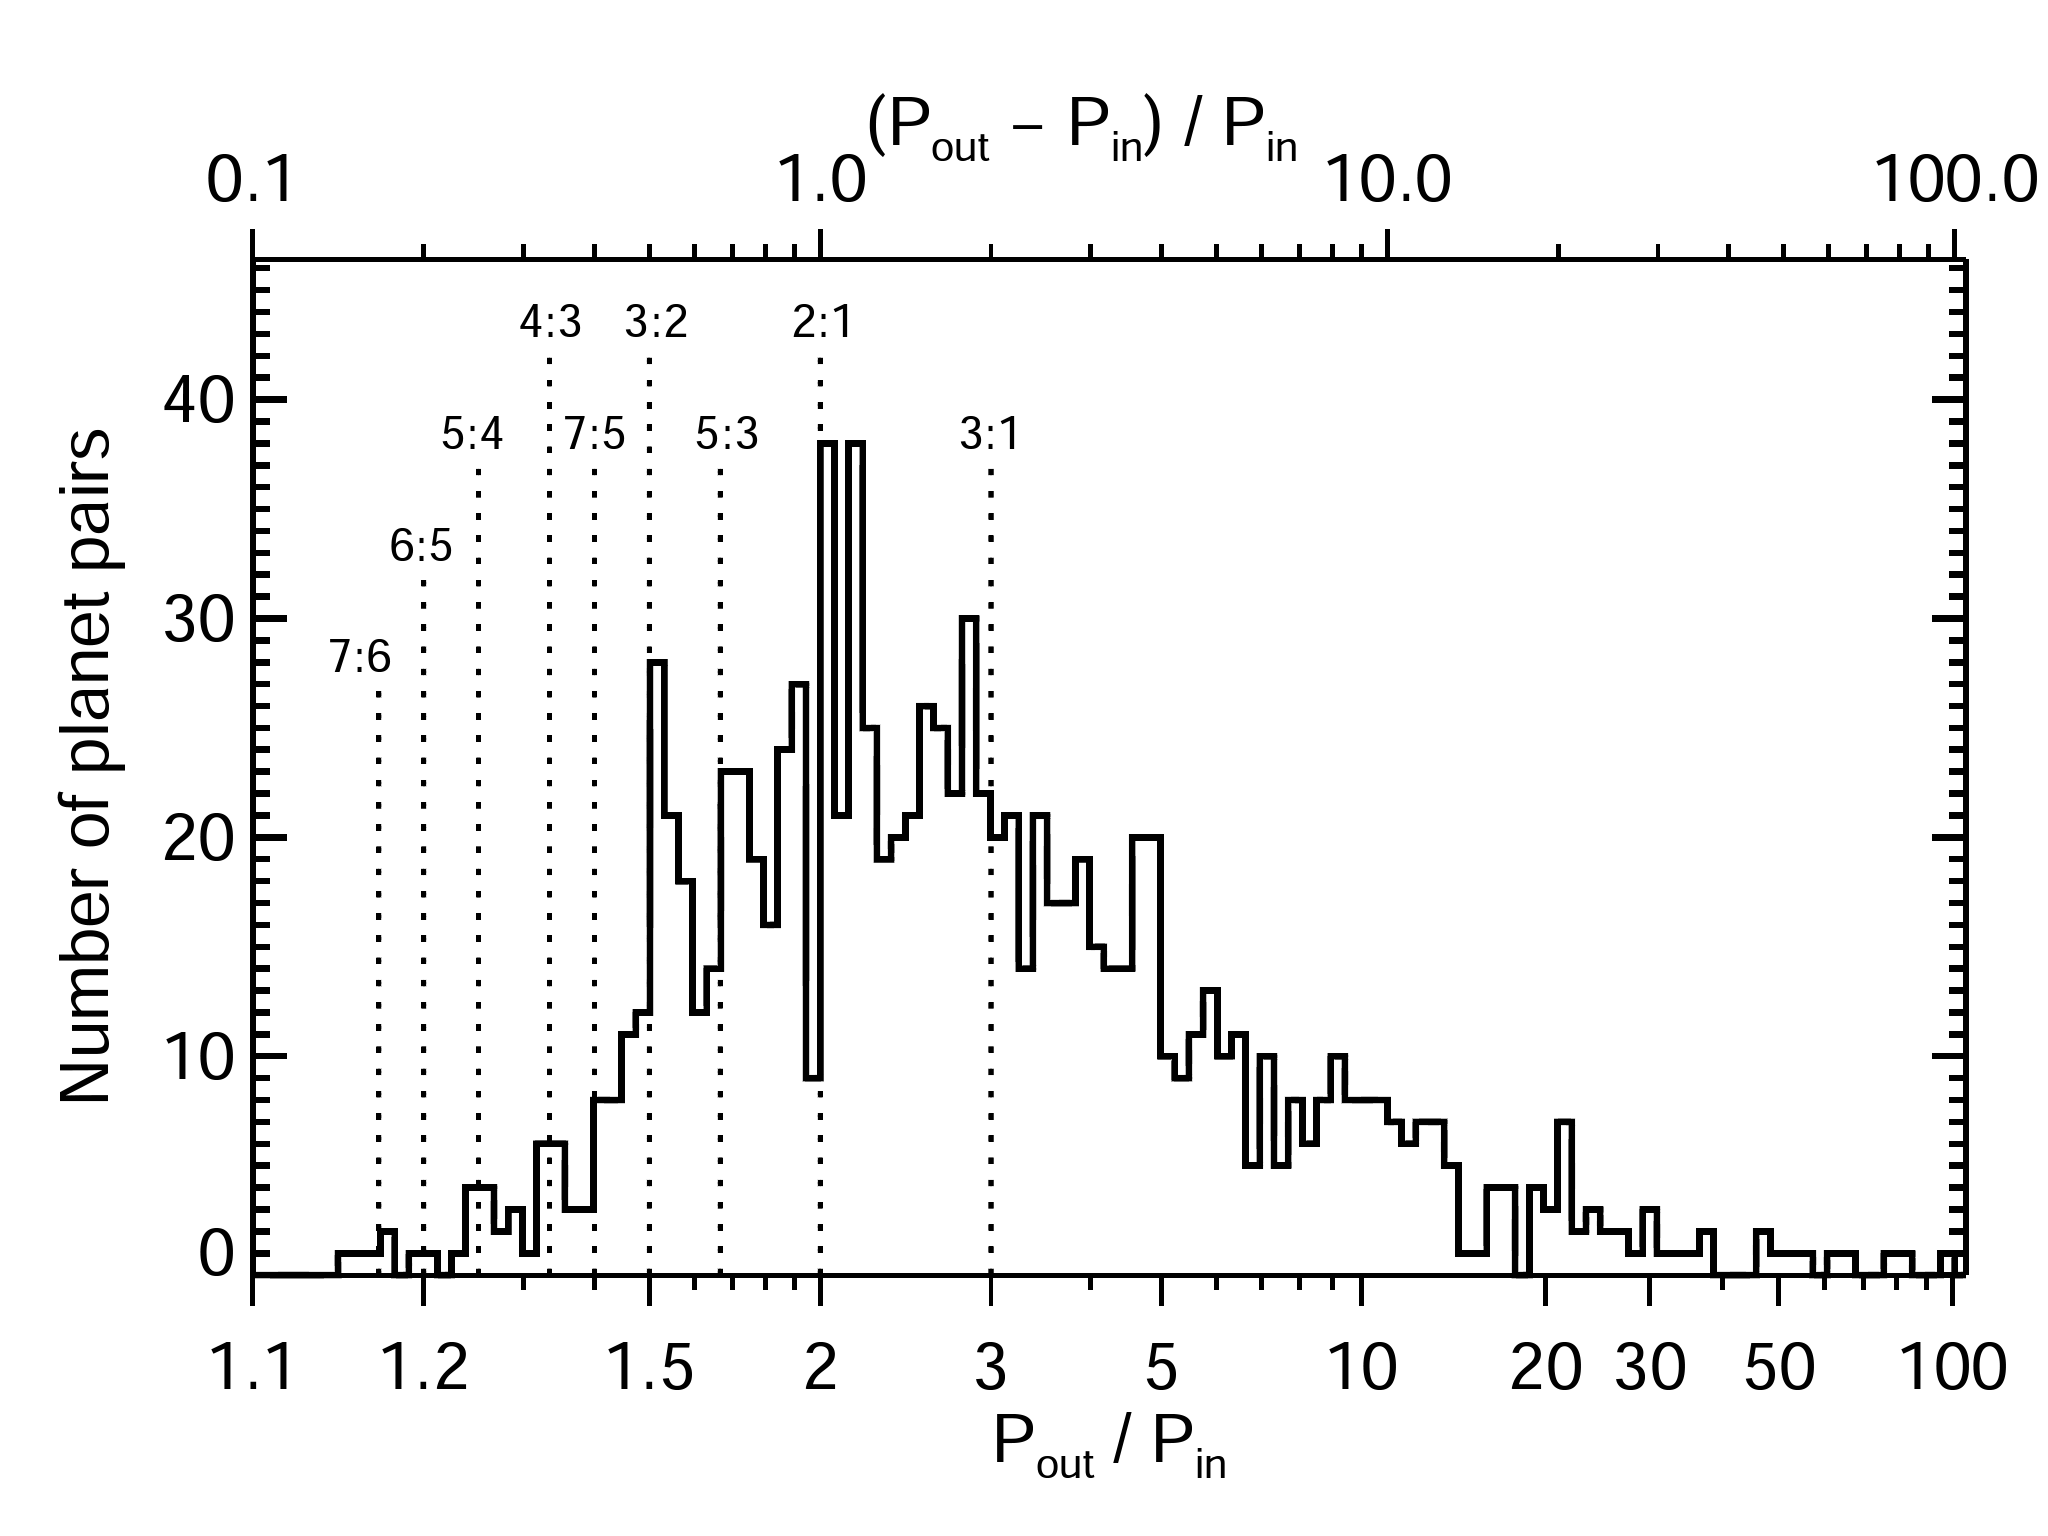
\includegraphics[trim={0cm 0 0 0},clip, width=0.9\textwidth]{exoresonance}
\caption{Da \cite{winnfabrycky15}.}\label{fig:exoresonance}
\end{subfigure}
~
\begin{subfigure}[b]{0.47\textwidth}
\centering
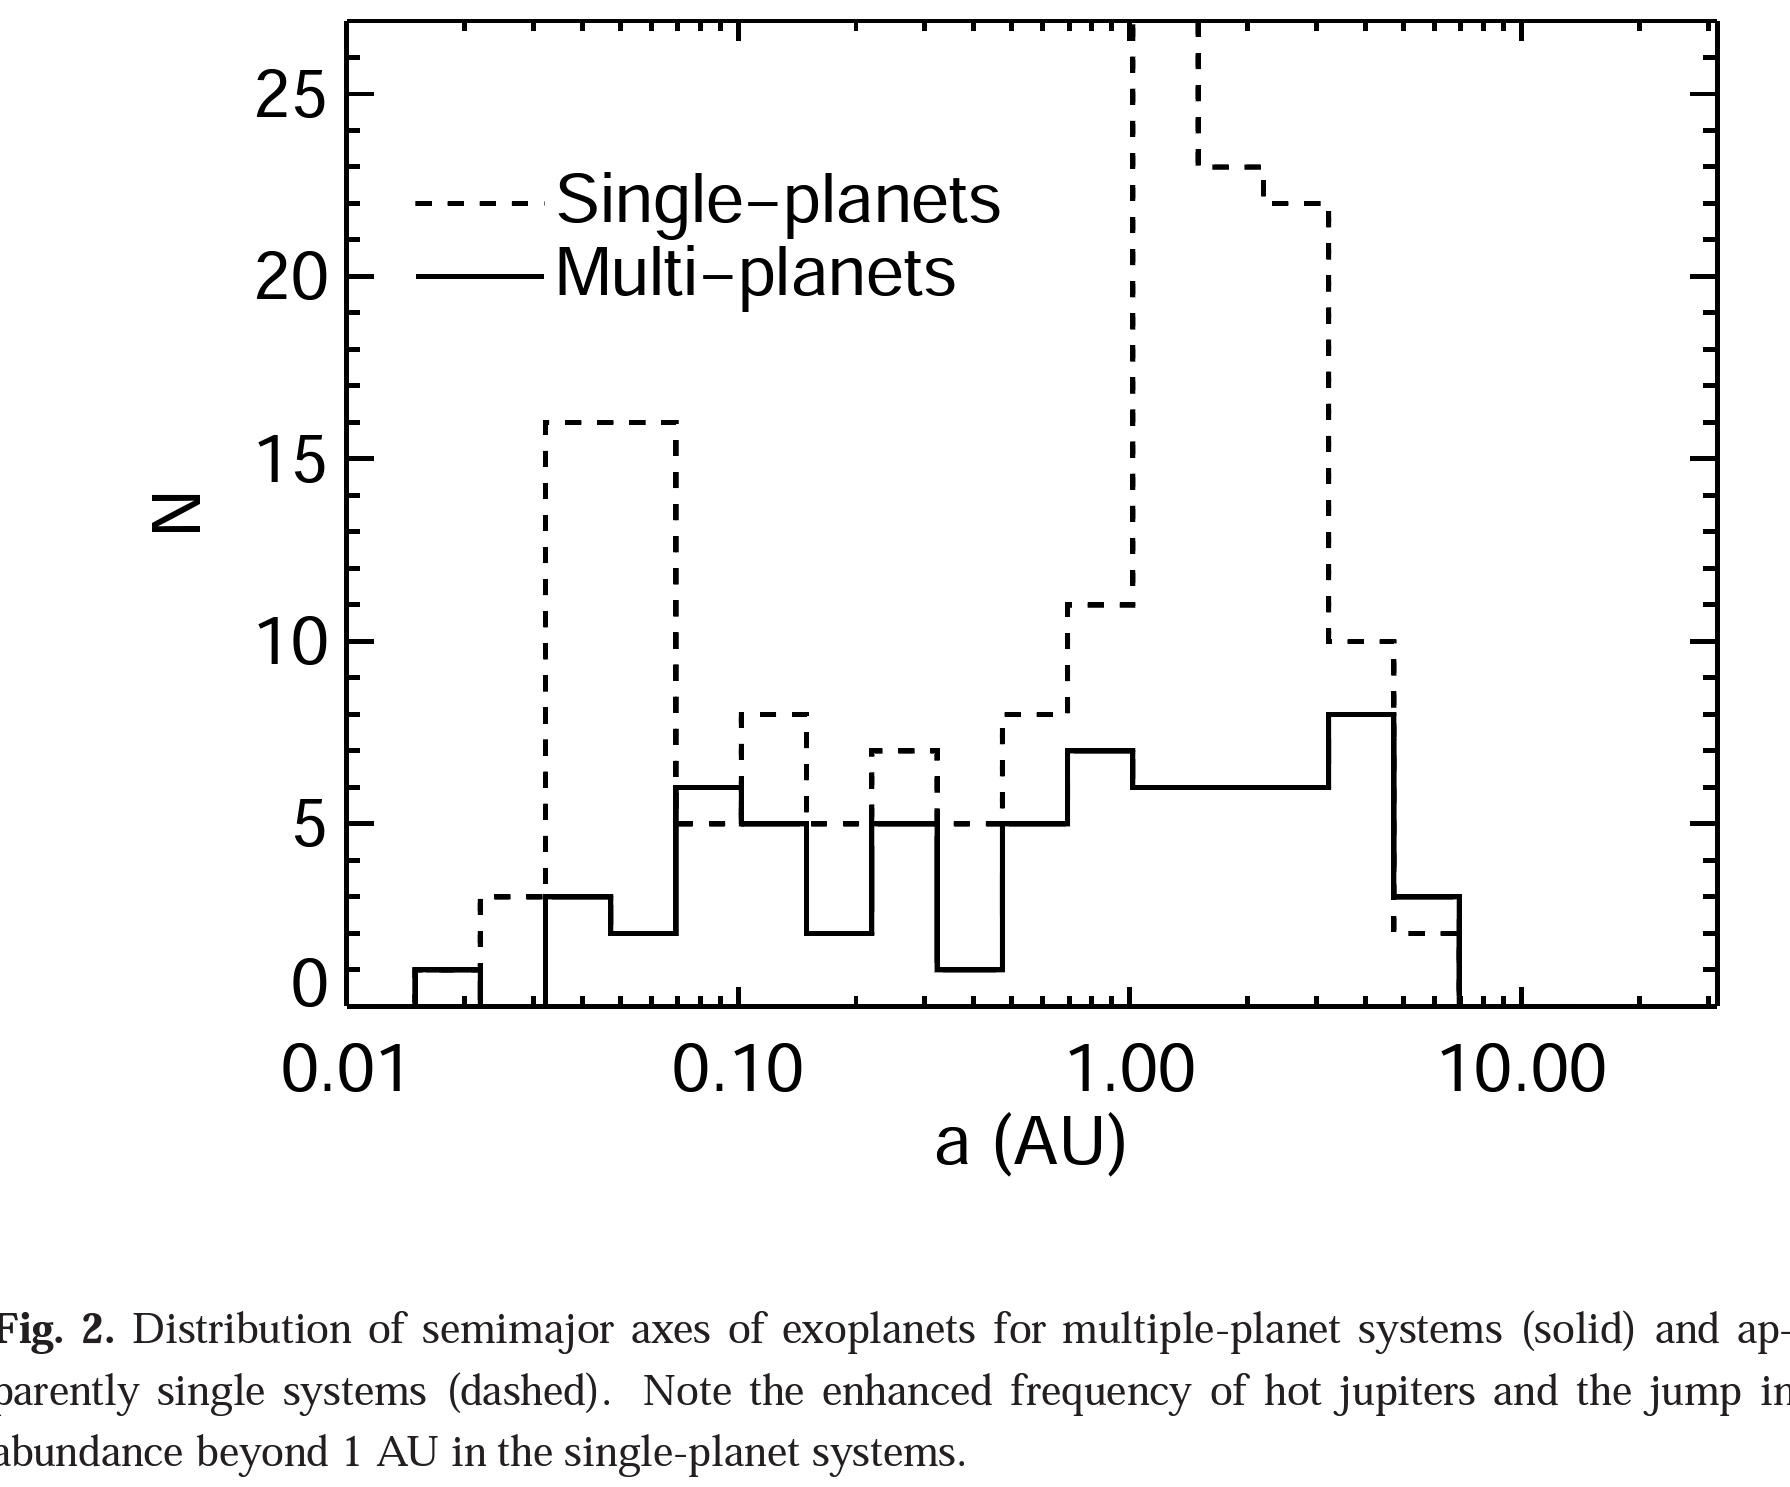
\includegraphics[trim={0cm 0 0 0},clip,width=0.9\textwidth]{singlemulti}
\caption{Da \cite{wright09}.}\label{fig:singlemulti}
\end{subfigure}
\end{figure}
\end{workout}

\begin{workout}[eccentricity distro: occurrence and architecture]
wright 09: multiplanet system tend to havelower eccentricity,
Limbach turner 14: $e_m\propto N\expy{-1.2}$.
planet around metal rich star have higher e (dawson, murray-clay 13)
smaller planets tend to have lower e (hogg 10 raccomanded modelling e distro on basis of Bayesian analysis)
\end{workout}f

\clearpage

\section{Popolazione esopianeti rilevati tramite transito}

Le osservabili sono la differenza di luminosit\'a durante il transito, la durata totale e di massima occultazione del transito, e il periodo: da questi \'e possibile ricavare $R_p$, a, i, $R_*$, $M_*$ facendo uso della relazione massa raggio appropriata per la fase evolutiva della stella, per stelle di sequenza principale
\begin{equation}
\frac{R_*}{\rsun{}}=(\frac{M_*}{\msun{}})\expy{0.8}
\end{equation}

La probabilit\'a che l'orbita di un pianeta sia allineata con l'osservatore in maniera da avere un transito \'e:
\begin{equation}
p=(\frac{R_*\pm R_p}{a})(\frac{1}{1-e^2})
\end{equation}
dove $\pm$ indica inclusione/esclusione di transiti a raso.
La maggiore probabilit\'a di transito per orbite eccentriche \'e compensata approssimativamente dalla minore probabilit\'a di rilevamento per la minor durata del transito.
In forma adimensionale l'equazione precedente si riscrive:
\begin{equation}
p=0.005(\frac{R_*}{\rsun{}})(\frac{a}{1AU})\expy{-1}(\frac{1}{1-e^2})
\end{equation}

Considerando un numero totale di osservazioni $N_o$ durante il transito si hanno $N_t\approx N_o\frac{R_*}{\pi a}$; il rapport segnale rumore \'e $S/N=\sqrt{N_t}\frac{\delta}{\sigma}$, $\sigma$ precisione fotometrica e $\delta=(\frac{R_p}{R_*})^2$. Per osservazione limitata da statistica fotoni $\sigma\propto\frac{1}{\sqrt{N_{ph}}}\propto d$: fissato S/N (e tipo stellare) il numero di pianeti rivelati varia come volume a cui \'e estesa la ricerca per probabilit\'a di transito:
\begin{equation}
V_p*P\propto d^3*\frac{R_*}{a}\propto R_p^6/P\expy{\frac{5}{3}}
\end{equation}

\begin{figure}[!ht]
\begin{subfigure}[b]{0.47\textwidth}
\centering
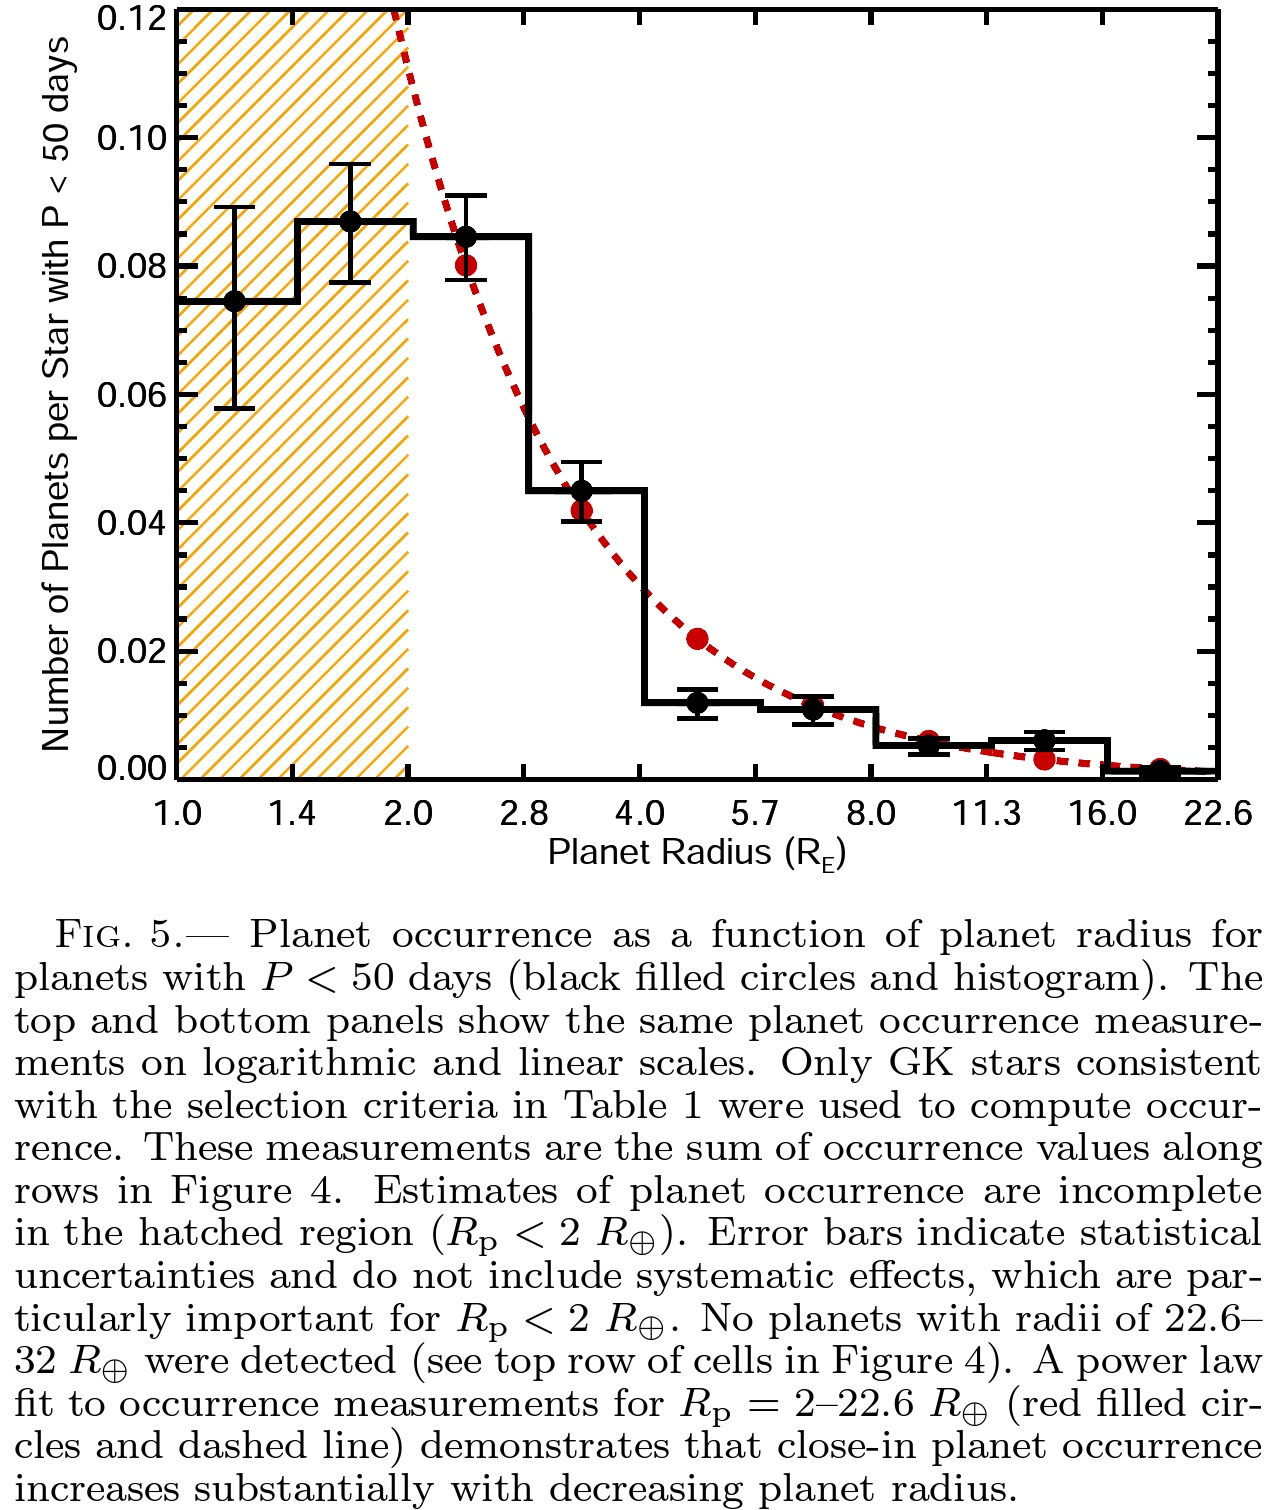
\includegraphics[trim={0cm 22cm 0 0},clip, width=0.95\textwidth]{freqvsRpl50d}
\caption{Distribuzione raggi planetari: crescita esponenziale verso piccoli raggi. La regione barrata indica misure incomplete. Da \cite{howard2012planet}.}\label{fig:howard2012planet}
\end{subfigure}
~
\begin{subfigure}[b]{0.5\textwidth} \centering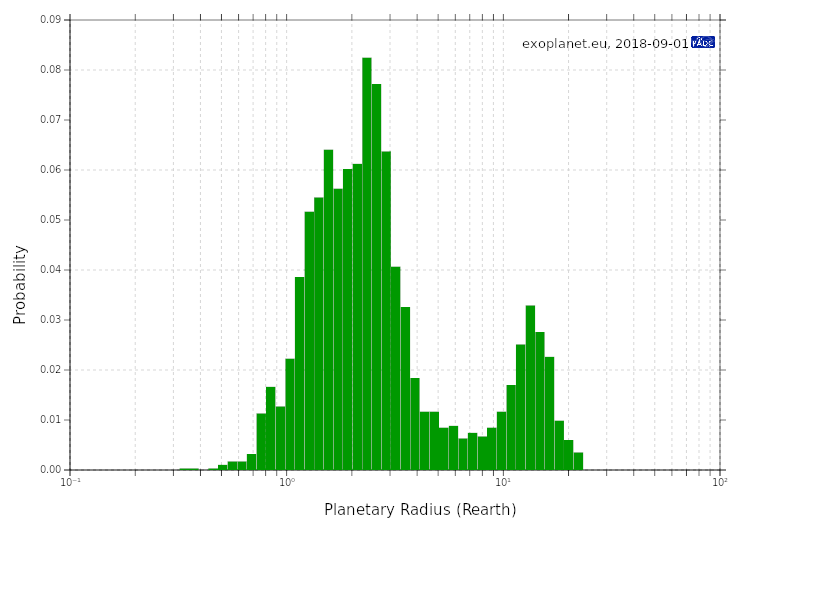
\includegraphics[trim={0cm 0.5cm 0 0},clip, keepaspectratio,width=0.99\textwidth]{probvsR-T}\caption{Distribuzione radiale pianeti rivelati tramite T. Da \cite{exoplanet.eu} (luglio 2018): la frequenza ha andamento crescente verso pianeti di raggio terrestre, andamento piatto tra $4-10\rearth{}$ e picco a $R\approx\rjupiter{}$.}\label{fig:probvsR-T}
\end{subfigure}
\end{figure}

La figura (\subref{fig:howard2012planet}) mostra distribuzione radiale corretta per probabilit\'a di transito; a fianco la distribuzione dei raggi planetarii aggiornata a Luglio 2018. 
%\begin{align*}
%&\TDy{\log{R}}{f}=k_RR\expy{\alpha}\\
%&k_R=2.9_{-0.4}^{+0.5},\ \alpha=-1.92\pm0.11
%\end{align*}

\begin{wrapfigure}[18]{l}{0.61\textwidth}
\centering 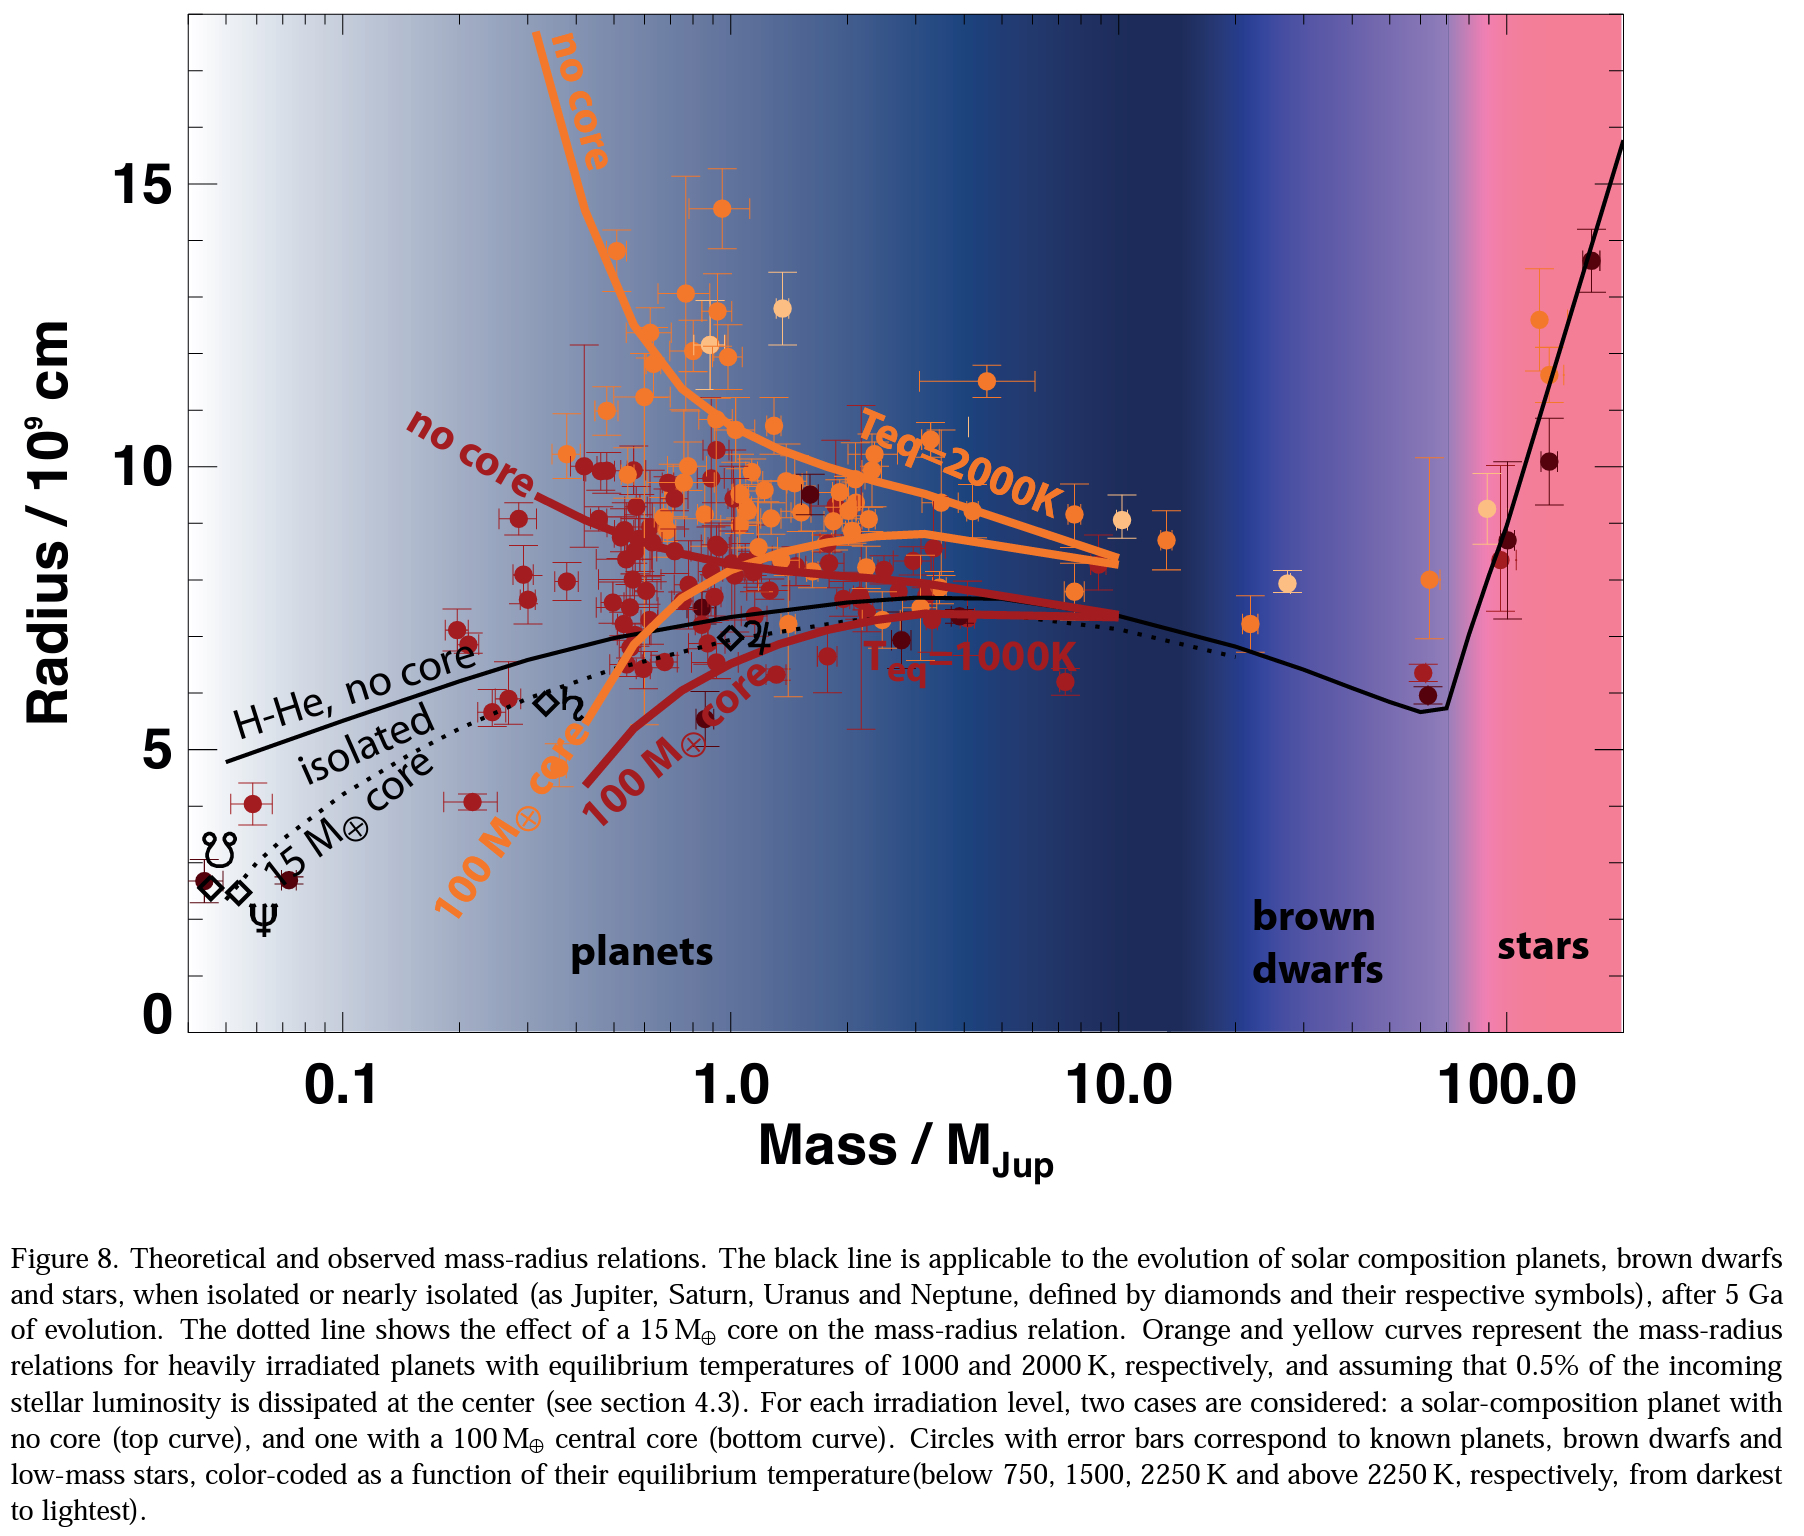
\includegraphics[trim={0cm 12cm 0 0},clip, width=0.6\textwidth]{MR-model-obs}
\caption{Relazione massa-raggio determinata sulla base di modello planetario dopo \SI{5}{\giga\year}. Per gli esopianeti sono indicate le curve per temperature di equilibrio di \SI{1000}{\kelvin} e \SI{2000}{\kelvin}. Da \cite{guillot2014giant}.}\label{fig:MR-model-obs}
\end{wrapfigure}

Nel caso un pianeta osservato tramite transito abbia massa nota \'e possibile determinarne la struttura interna tramite un modello planetario: La posizione di un pianeta nel diagramma massa-raggio \'e determinata dalla storia di accrescimento del pianeta (pianeta roccioso, pianeta costituito in parte da ghiacci, pianeta con massa consistente di gas), dal bilancio termico, e propriet\'a di H/He e metalli a alte densit\'a (rottura H molecolare, ionizzazione da pressione, degenerazione elettronica, transizioni di fase). La figura \ref{fig:MR-model-obs} mostra la relazione massa-raggio per pianeti nettuniani fino a regimi stellari. Considerando l'equazione di stato
\begin{equation}
P\propto\rho\expy{\gamma},\ \gamma=\frac{1}{n}+1
\end{equation}
la relazione massa raggio \'e
\begin{equation}
R\propto M\expy{(1-n)/(3-n)}
\end{equation}
per $M\approx\mjupiter$ $n\approx1$ quindi il raggio \'e approssimativamente costante. Questo fatto \'e visibile anche nella distribuzione dei raggi planetari (figura \subref{fig:probvsR-T}) nel picco attorno a $\rjupiter$.
La figura (\subref{fig:RfreqPl100ub}) mostra due picchi nella distribuzione radiale a $1.3\rearth{}$ e $2.4\rearth{}$ dovuti alle sottopopolazioni di pianeti rocciosi e gassosi per $P<\SI{100}{\day}$: i pianeti rocciosi hanno atmosfera di H/He che non contribuisce alle dimensione mentre i pianeti nettuniani hanno strato di gas consistente rispetto alla massa del pianeta. La valle a $1.7\rearth{}$ potrebbe essere il raggio di separazione tra pianeti terrestri con atmosfera tenue di H/He soggetta a evaporazione e pianeti nettuniani con massa consistente di H/He.
La distribuzione dei periodi \'e mostrata in figura (\subref{fig:freqperstarvsPanfit}): i pianeti sono raggruppati per intervalli di raggio. La frequenza dei pianeti in funzione del periodo segue andamento
\begin{equation}
\TDy{\log{P}}{f}=K_PP\expy{\beta}[1-\exp{-(\frac{P}{P_0})\expy{\gamma}}]
\end{equation}
Si ipotizza che il diverso valore del raggio critico $P_0$ (riportato in figura) sia dovuto alla dipendenza dal raggio planetario del meccanismo di frenamento della migrazione.

\begin{errata}[Equazione di stato politropa: relazione massa raggio]
\begin{equation}
P\propto\rho\expy{\gamma},\ \gamma=\frac{1}{n}+1
\end{equation}
si che per $M\approx\mjupiter$ $n\approx1$.
Inoltre la relazione massa-raggio  \'e approssimabile
\begin{equation}
R\propto M\expy{(1-n)/(3-n)}
\end{equation}
\end{errata}

%\begin{figure}[!ht] \centering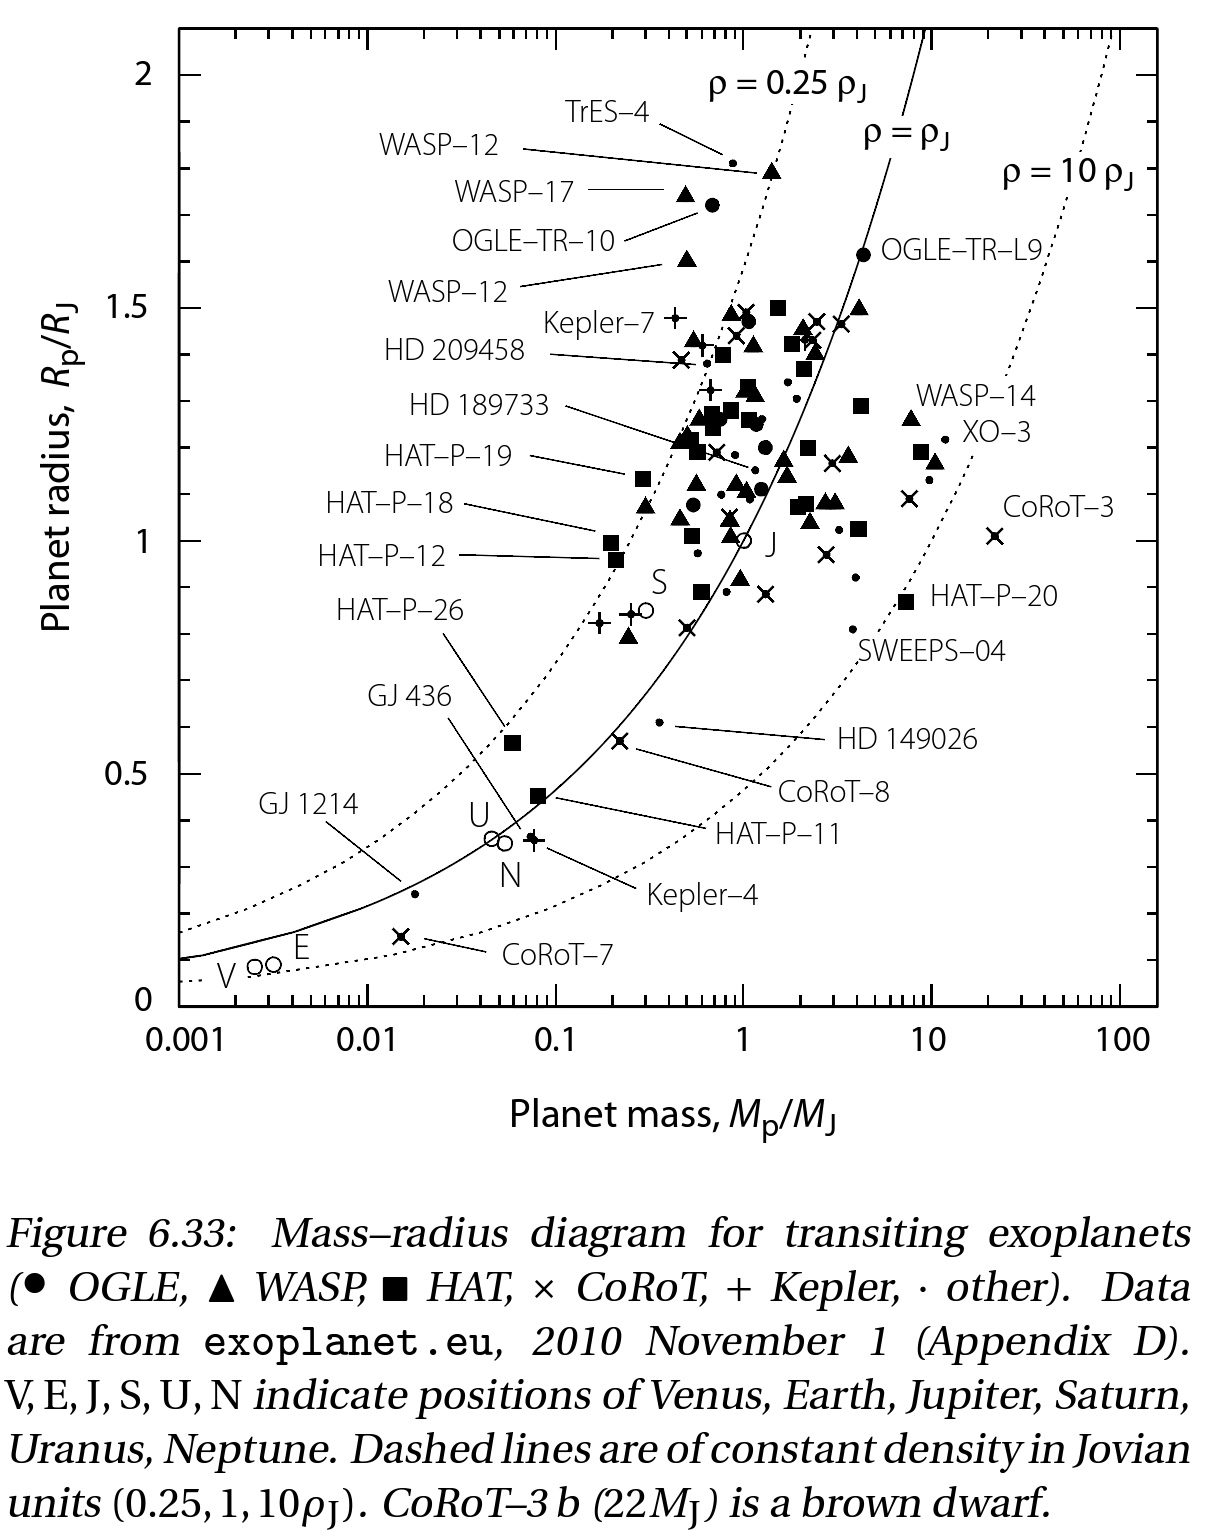
\includegraphics[trim={0cm 14cm 0 0},clip, keepaspectratio,width=0.9\textwidth]{MRD}\caption{Diagramma mass-raggio per pianeti di transito. Le curve tratteggiate sono a densit\'a costante. Il simbolo $\circ$ indica i pianeti del sistema solare. Da \cite{perryman2011exoplanet}.}\label{fig:MRD}
%\end{figure}

%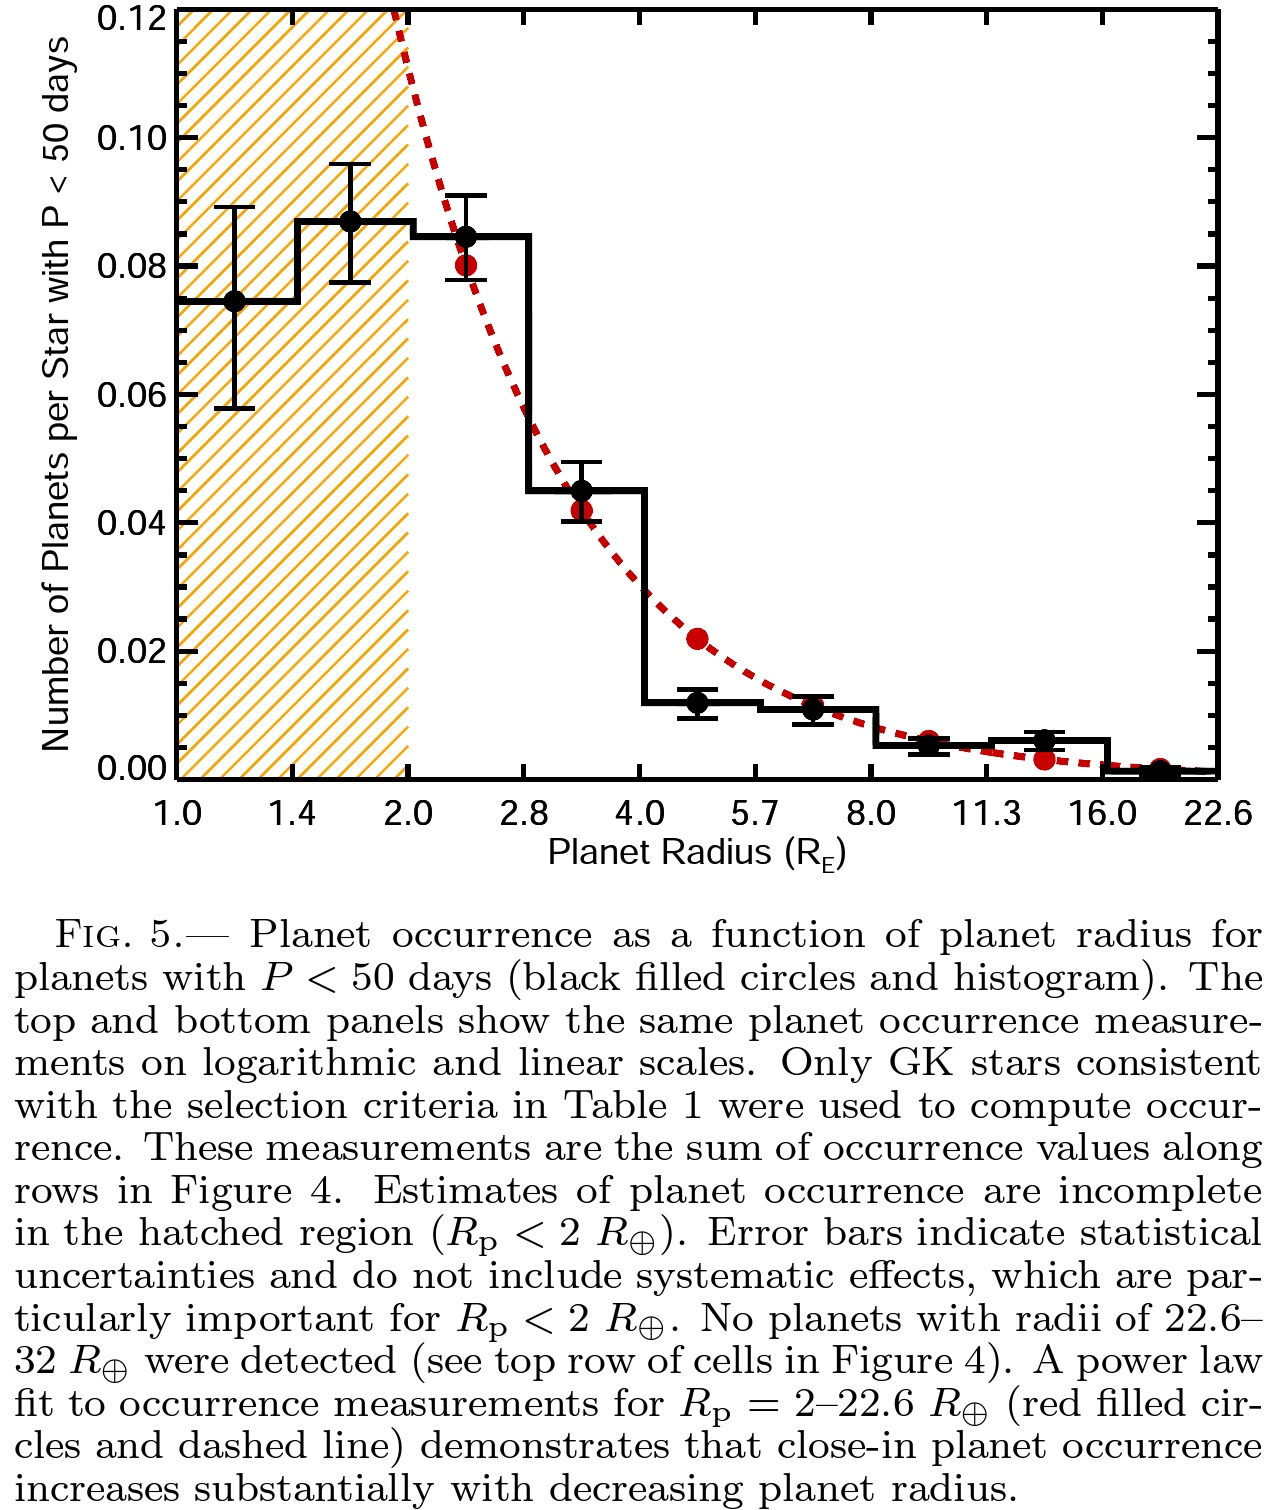
\includegraphics[trim={0cm 0 0 0},clip, keepaspectratio,width=0.9\textwidth]{freqvsRpl50d}\label{freqvsRpl50d}\caption{Da \cite{howard2012planet}}
% 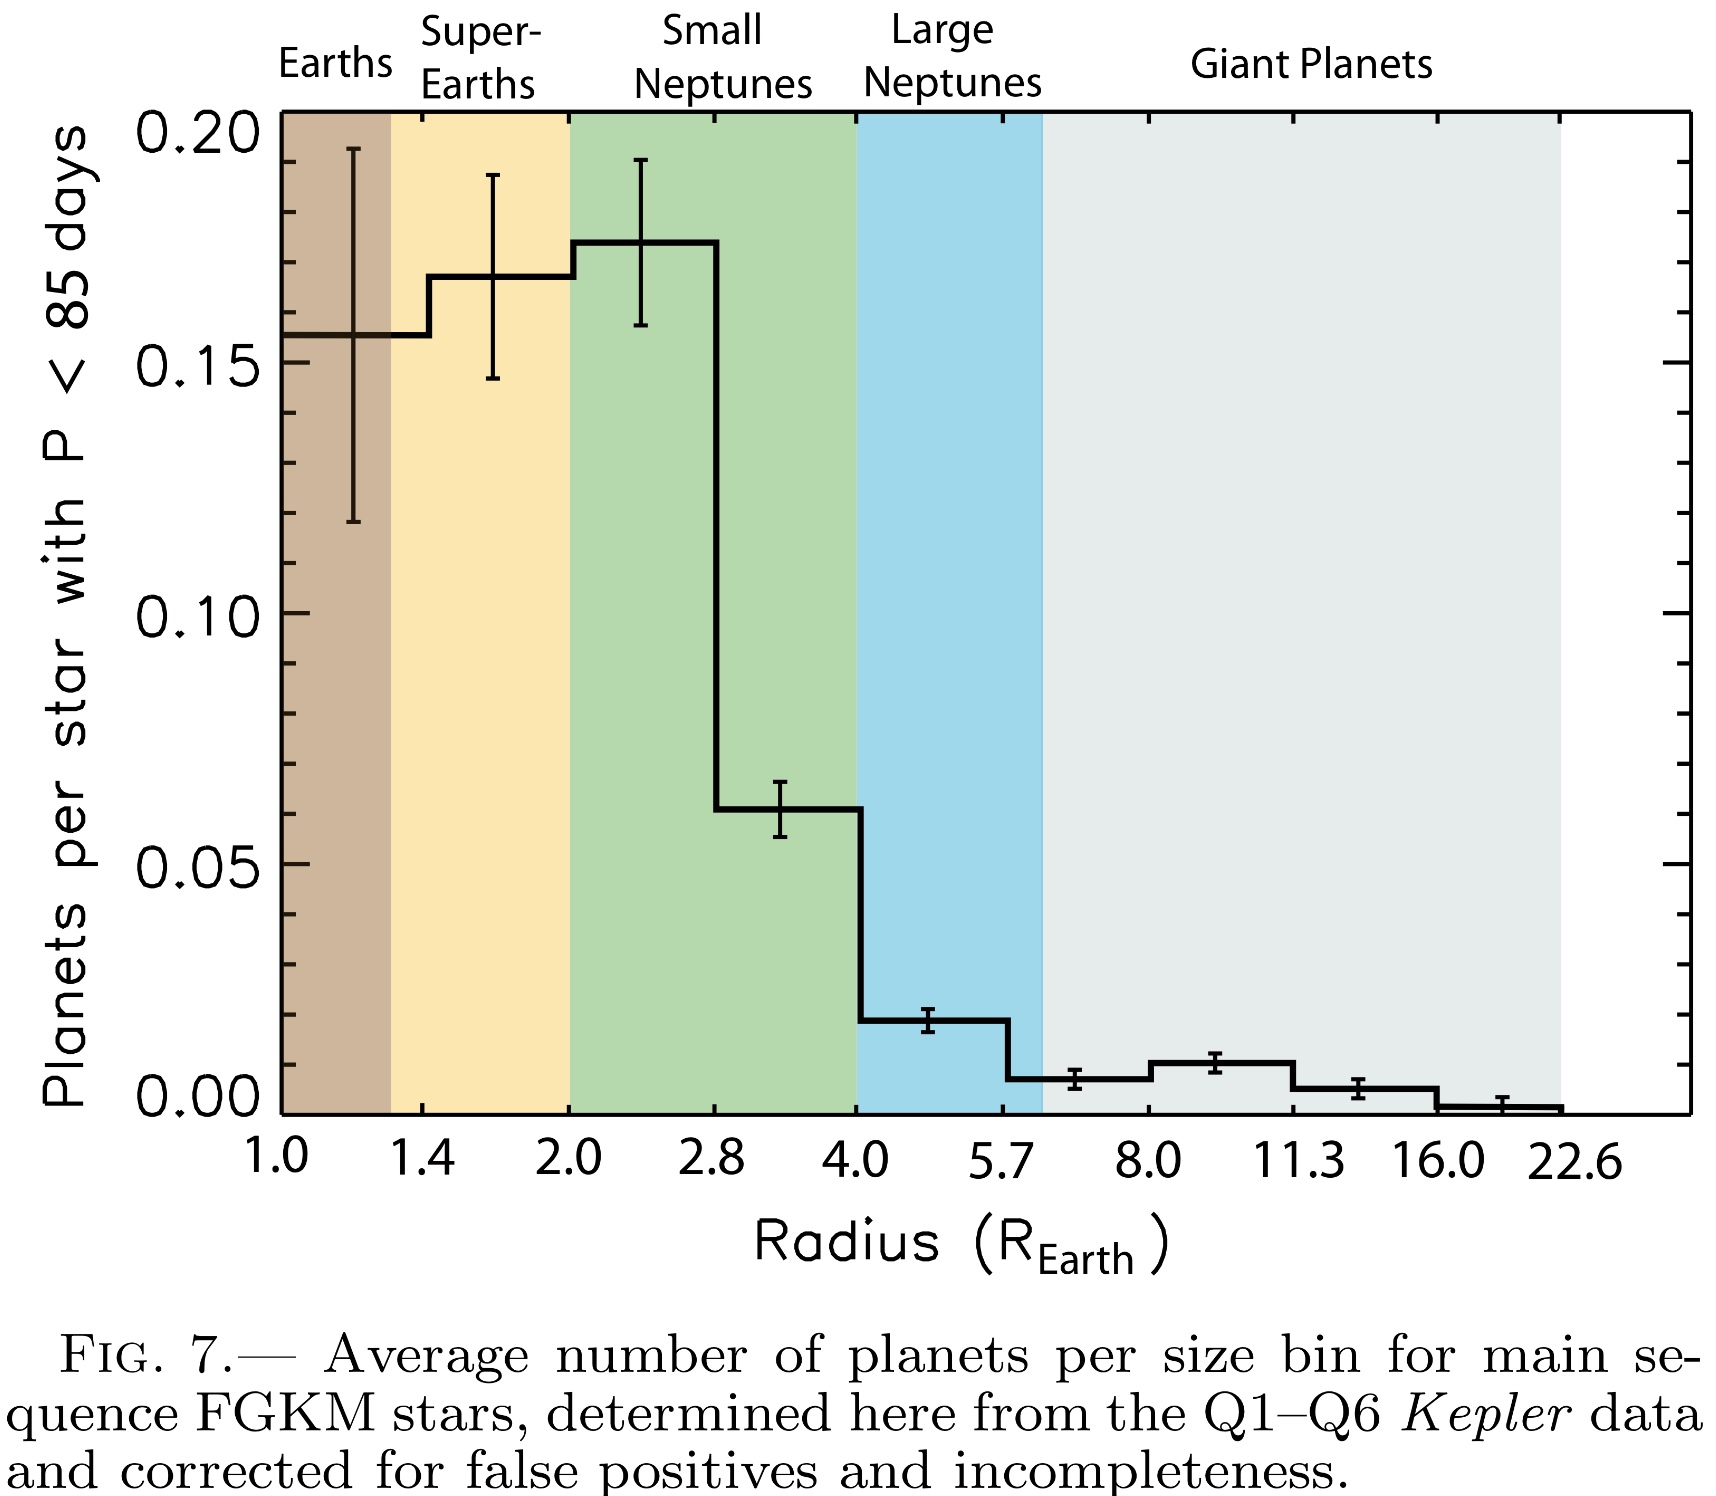
\includegraphics[trim={0cm 0 0 0},clip,width=0.95\textwidth]{keplerRfreq}\label{fig:keplerRfreq} \caption{Da \cite{fressin2013false}}
%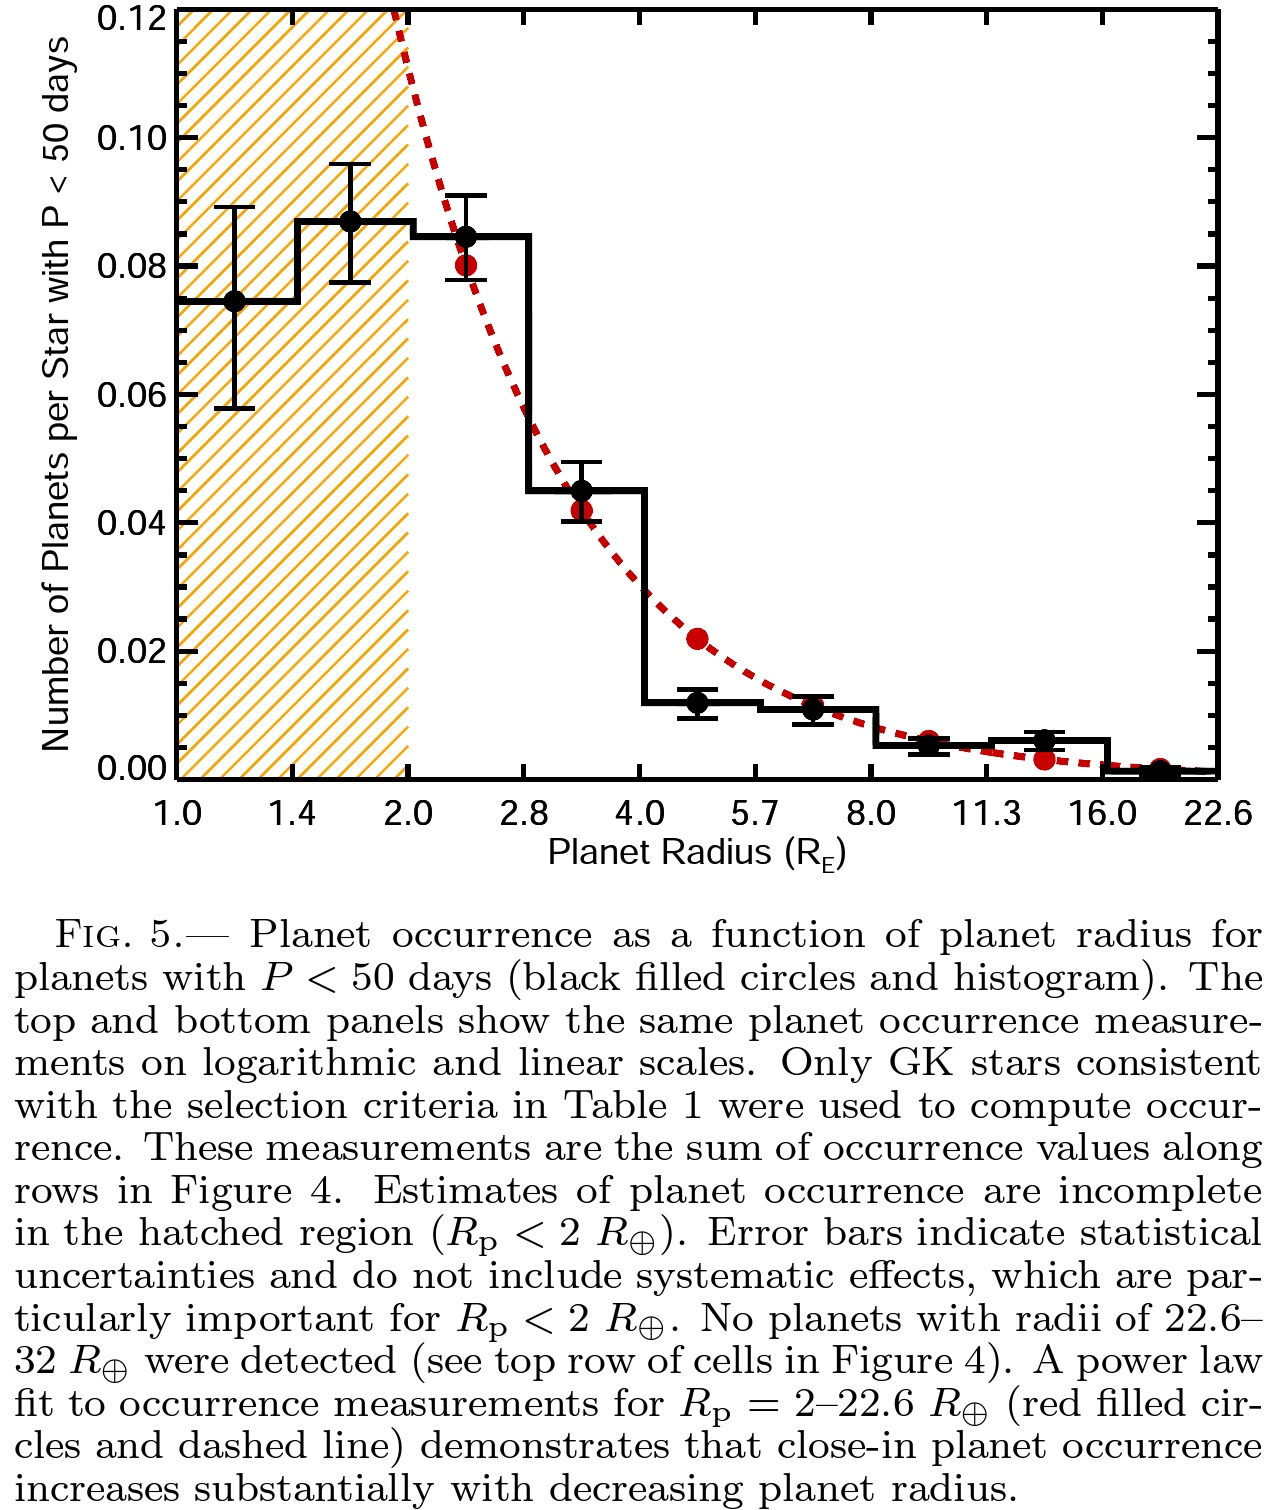
\includegraphics[trim={0cm 0 0 0},clip, keepaspectratio,width=0.9\textwidth]{freqvsRpl50d}\label{fig:freqvsRpl50d}\caption{Da \cite{}.}

\begin{figure}[!ht]
\begin{subfigure}[b]{0.49\textwidth} \centering 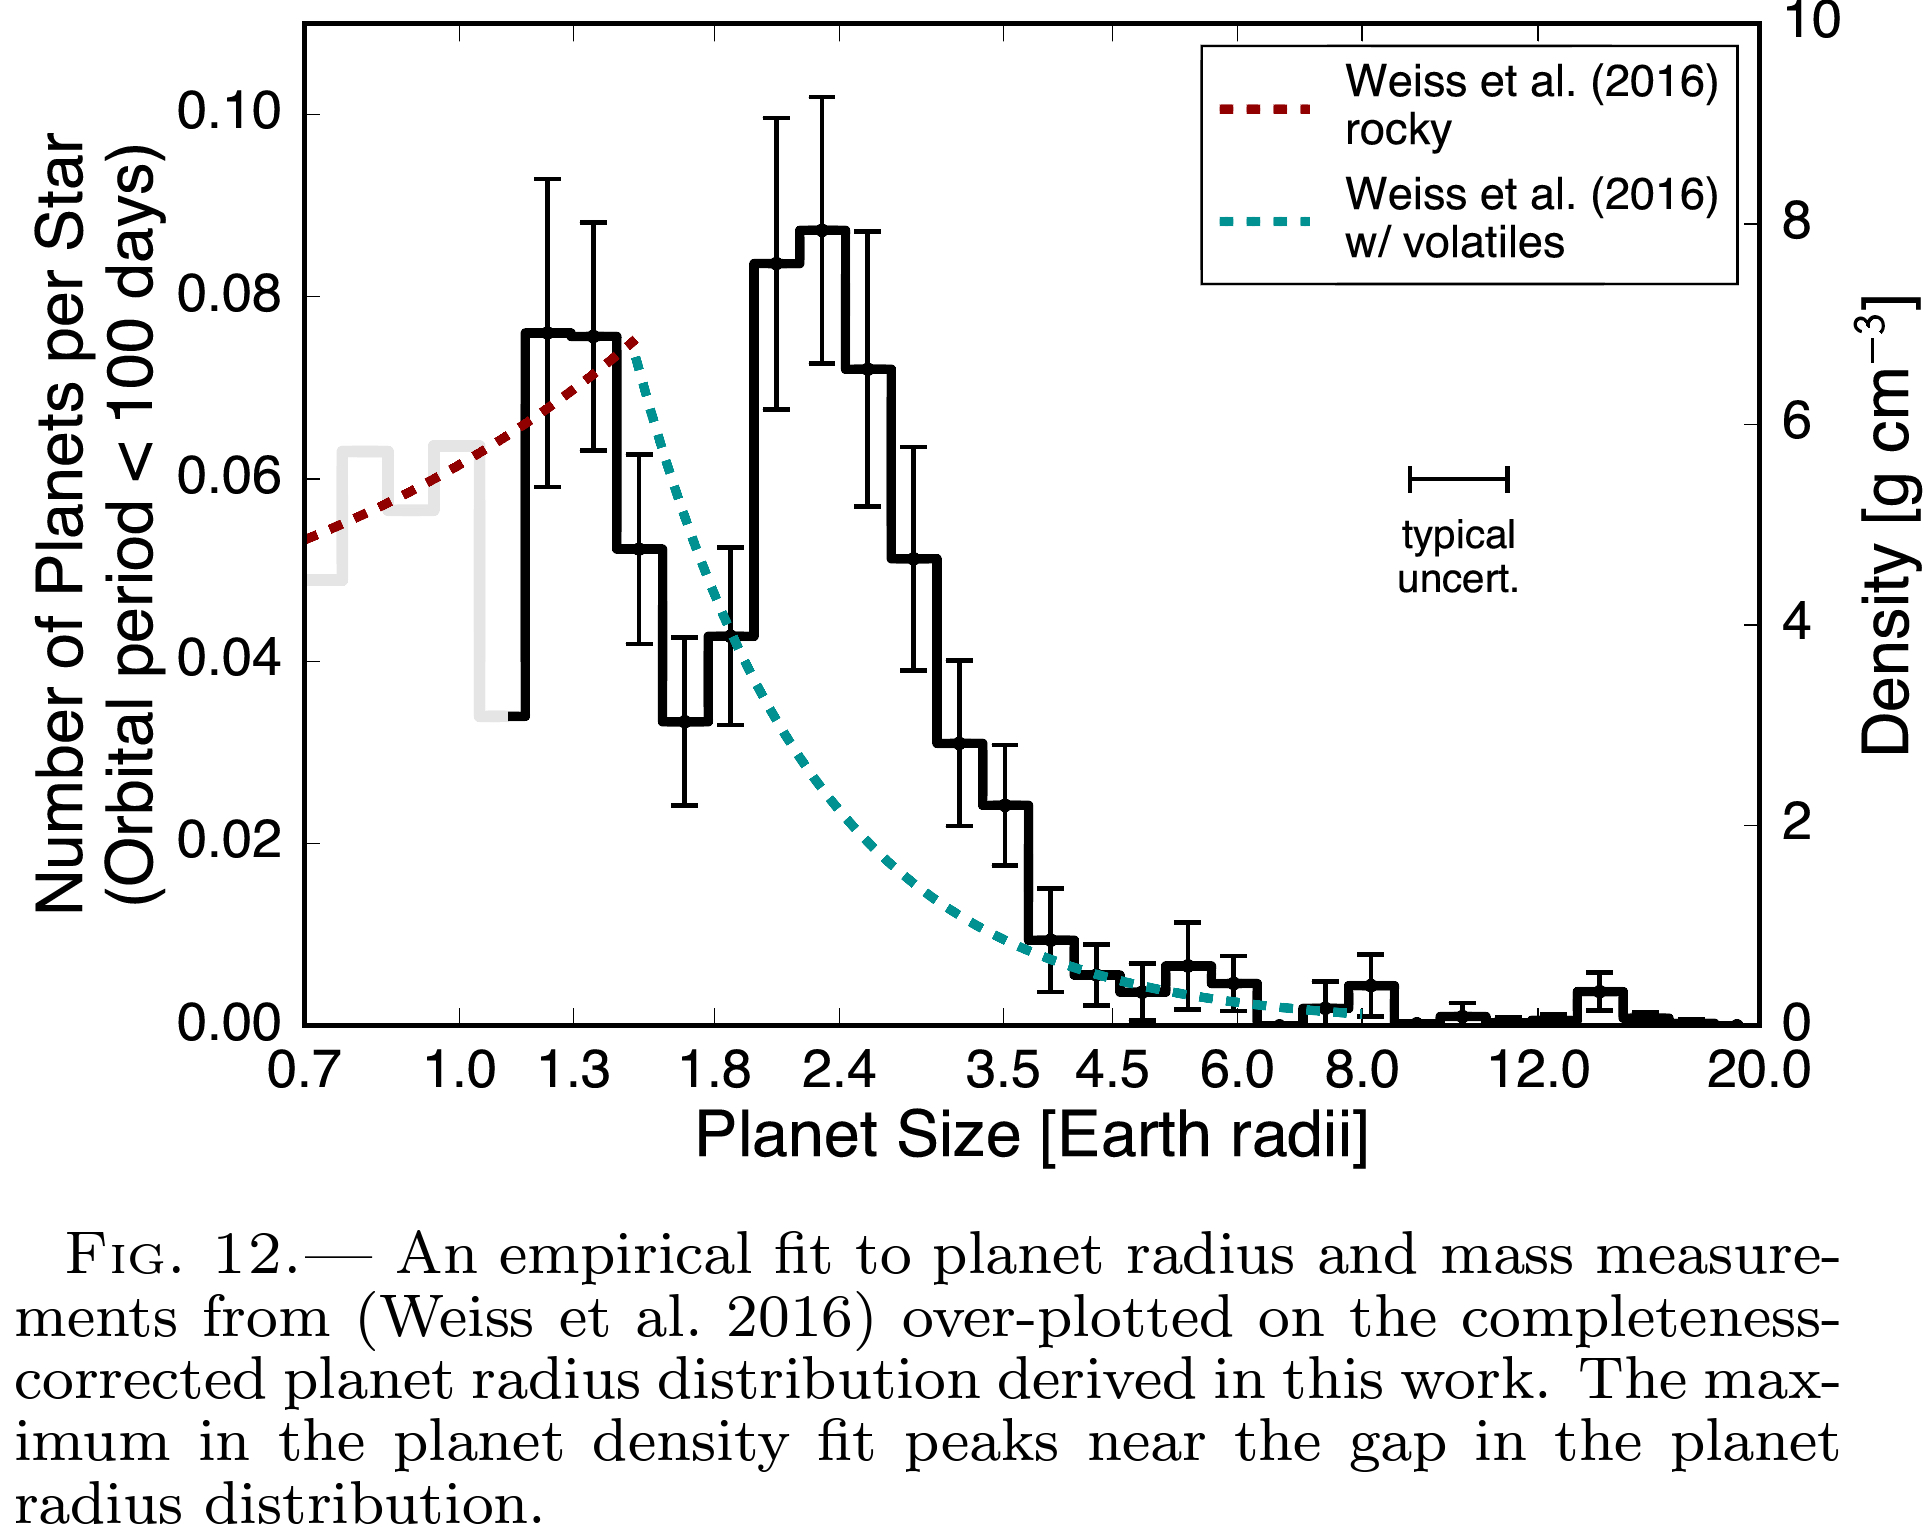
\includegraphics[trim={0 12cm 0 0},clip, width=0.95\textwidth]{RfreqPl100ub} 
\caption{Distribuzione per i pianeti osservati tramite transito con $P<\SI{100}{\day}$: la valle a $1.7\mearth{}$ si ipotizza causato dall'evaporazione. Da \cite{fulton2017california}.}\label{fig:RfreqPl100ub}\end{subfigure}
~
\begin{subfigure}[b]{0.47\textwidth}
\centering
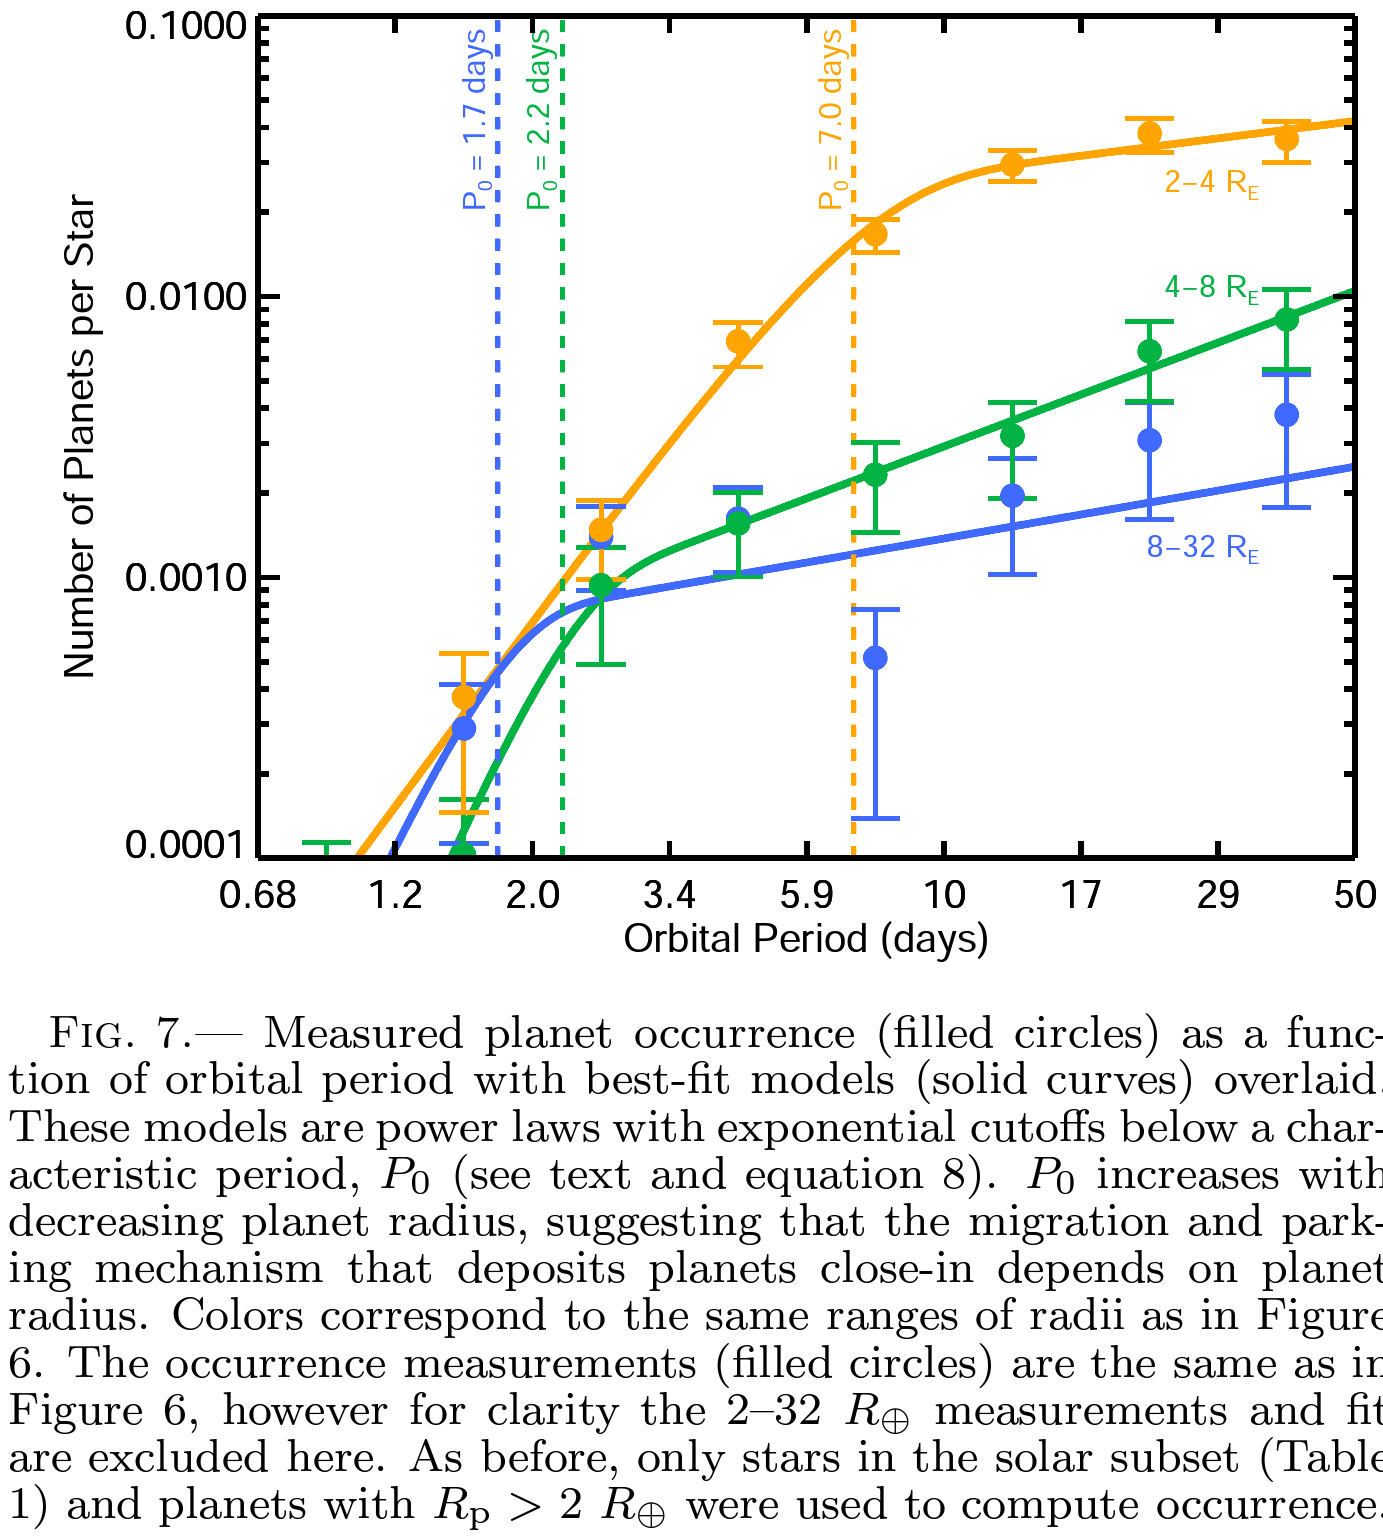
\includegraphics[trim={0cm 19cm 0 0},clip,width=0.95\textwidth]{freqperstarvsPanfit}
\caption{Distribuzione dei periodi orbitali raggruppate per diversi raggi planetari: indicato il diverso periodo critico a cui si ha drastica diminuzione nella distribuzione planetaria. Da \cite{howard2012planet}.}\label{fig:freqperstarvsPanfit}
\end{subfigure}
\end{figure}

\begin{workout}[transit distro observed refs]
Refs:Mthods of detecting exoplanets (radius distro: pg 136)
the occurrence within 0.25 au of solar-type stars from kepler
occurrence architecture exoplanetary
fressin 13: 
petigure 13: plateau PLANET POPULATION BELOW TWICE EARTH SIZE
bathala 13
exoplanet.eu
\end{workout}

\begin{workout}[radius distro]
Local maximum at $1\mjupiter{}$, flat distro in log(r) between $4-10\mearth{}$ below strong increase, at $1.7\mearth{}$ local minimum separating super-earth from sub-neptune
\end{workout}

\begin{workout}[planet model: relazione massa-raggio]
characterization of exoplanets from formation: MR relation pg 18
formazione: vedi \ref{ch:gasaccretion}
MR diagram chabrier 09 (perryman 143)
\end{workout}

\begin{workout}[KEPLER MULTI-PLANET SYSTEM]
THE CALIFORNIA-KEPLER SURVEY. V. PEAS IN A POD: PLANETS IN A KEPLER MULTI-PLANET SYSTEM ARE SIMILAR IN SIZE AND REGULARLY SPACED
						 III - A gap in radius distribution of small planets
\end{workout}

\begin{workout}[transiti refs: osservabilie probabilit\'a di rilevamento]
pg103
pg 117, eccentric orbit pg 121-122
From space: presence of structure on stellar surface Perryman 3.4, Eriksson Lindegren 07; simulation of stellar jitter: Svensson Ludwig 05, Ludwig 06.
Probability of randomlyoriented planet on circular/eccentric orbit (Borucki Summers 84/Barnes 07, Burke 08,  Seagroves 03, Kane von Braun 08):
\end{workout}

\begin{workout}[Transiti: Propriet\'a dei pianeti a transito]
pg 143, fig 6.33, 6.34, 6.35
Mass-radius relation: chabrier 09
\end{workout}

\begin{workout}[M-R diagram]
orbital migration 10.8 Perryman, tidal effect 10.9, 
fig11.2, 11,4 (EOS), 11.7, 11.8 (M-R)
Ternary diagram 11.9, M-R realtion
Fig 6.33/34/35: mass radius realtion

pg 144: theoretical model - La posizione di un pianeta nel diagramma M-R fornisce indicazione della composizione
fig 6.35
\end{workout}

\begin{workout}[Struttura orbitale e risonanze moto medio]
\end{workout}

\begin{workout}[Long term dynamical stability: mmr, fully packing, eccentricity, inclination distro]
tidal circularization
resonance capture and migration (pg 41)
barnes 08: secularly/resonant dominated
Planets near mmr (Petrovich 12): strength of resonance
P-P scattering leds to tightly packed planetary systems (Raymond barnes 09)
Architecture of planetary systems based om kepler data: number of planets and coplanarity (Fang Margot 12): e,i distro.
Spacing Kepler planets (Wu Pu 15)
Are planetary systems filled to capacity? (Fang Nargot 13)
\end{workout}
